%
%  Halibut
%
%  Created by Martell on 2012-03-05.
%  Copyright (c) 2012 UBC Fisheries Centre. All rights reserved.
%
\documentclass[12pt]{report}
\usepackage[round]{natbib}
% Use utf-8 encoding for foreign characters
\usepackage[utf8]{inputenc}

% Setup for fullpage use
\usepackage{fullpage}

% Uncomment some of the following if you use the features
%
% Running Headers and footers
\usepackage{fancyhdr}

% Multipart figures
%\usepackage{subfigure}

% More symbols
\usepackage{amsmath}
\usepackage{amssymb}
\usepackage{latexsym}

% Surround parts of graphics with box
\usepackage{boxedminipage}

% Package for including code in the document
\usepackage{listings}
\usepackage{alltt}
\usepackage{url}

% If you want to generate a toc for each chapter (use with book)
\usepackage{minitoc}

% This is now the recommended way for checking for PDFLaTeX:
\usepackage{ifpdf}

% -----------------------------------------------------------------------------
%% -math tables-
\newcounter{saveEq}
  \def\putEq{\setcounter{saveEq}{\value{equation}}}
  \def\getEq{\setcounter{equation}{\value{saveEq}}}
  \def\tableEq{ % equations in tables
    \putEq \setcounter{equation}{0}
    \renewcommand{\theequation}{T\arabic{table}.\arabic{equation}}
    \vspace{-5mm}
    }
  \def\normalEq{ % renew normal equations
    \getEq
    \renewcommand{\theequation}{\arabic{section}.\arabic{equation}}}

  \def\puthrule{ %thick rule lines for equation tables
    \hrule \hrule \hrule \hrule \hrule}
% -----------------------------------------------------------------------------

% -----------------------------------------------------------------------------
%Water mark
\usepackage{eso-pic}
%\usepackage{graphicx}
\usepackage{color}
\usepackage{type1cm}
\usepackage{float} 
\usepackage{array}
\makeatletter
  \AddToShipoutPicture{%
    \setlength{\@tempdimb}{.6\paperwidth}%
    \setlength{\@tempdimc}{.45\paperheight}%
    \setlength{\unitlength}{1pt}%
    \put(\strip@pt\@tempdimb,\strip@pt\@tempdimc){%
      \makebox(0,0){\rotatebox{45}{\textcolor[gray]{0.85}
      {\fontsize{2.00cm}{1.75cm}\selectfont{DRAFT \today}}}}
    }
} \makeatother
% -----------------------------------------------------------------------------


%\newif\ifpdf
%\ifx\pdfoutput\undefined
%\pdffalse % we are not running PDFLaTeX
%\else
%\pdfoutput=1 % we are running PDFLaTeX
%\pdftrue
%\fi

\ifpdf
\usepackage[pdftex]{graphicx}
\else
\usepackage{graphicx}
\fi

\title{Halibut Bycatch Management Research}
\author{ Steven J.D. Martell \\ University of British Columbia\\  2202 Main Mall, \\ Vancouver, BC\\ V6T 1Z4\\
%
\noindent\hrulefill\\
Document started March 5, 2012.
 }

\date{2012-03-05}

\begin{document}


\ifpdf
\DeclareGraphicsExtensions{.pdf, .jpg, .tif}
\else
\DeclareGraphicsExtensions{.eps, .jpg}
\fi

\pagenumbering{roman}
	\maketitle \thispagestyle{empty}
\thispagestyle{empty}
\clearpage


\newpage


%% -Executive summary material------------------------------------------

\pagenumbering{roman}
%!TEX root = /Users/stevenmartell/Documents/iSCAM-project/fba/Halibut/WRITEUP/Halibut.tex
\section*{Executive Summary} % (fold)
\label{sec:executive_summary}
\addcontentsline{toc}{section}{Executive Summary}

% section executive_summary (end)


\newpage
\tableofcontents
\addcontentsline{toc}{section}{Contents}
\newpage

\listoffigures
\addcontentsline{toc}{section}{List of Figures}
\newpage

\listoftables
\addcontentsline{toc}{section}{List of Table}
\newpage
%% -Main body of the document-------------------------------------------
\pagenumbering{arabic}



\part{Impacts of bycatch \& wastage on halibut yield}
\setcounter{chapter}{1}
cutoff%!TEX root = /Users/stevenmartell/Documents/CURRENT PROJECTS/iSCAM-trunk/fba/BC-herring-2011/WRITEUP/BCHerring2011.tex


\section{Introduction}

The objectives of this section of the report are: (1) present the data used in the 2011 assessment, (2) provide a summary overview of the integrated statistical catch-age model (hereafter, \iscam), (3) present the 2011 stock assessment and forecast for 2012, and (4) describe in detail the decision table used to provide advice to fisheries management.

BC herring are currently managed as five major stocks and 2 minor stocks (Figure \ref{Fig1}).  Annual catch advice for each of these areas is based on current estimates of stock status, and a 20\% exploitation rate if the post-fishery stock is above the cutoff level for the five major stocks and a 10\% exploitation rate for the two minor stocks.  Cutoff levels for the five major stocks historically were based on the 1996 estimate of  0.25$B_o$.  These cutoffs are currently thought to be more conservative 	than the suggested default Limit Reference Point of 0.4\bmsy\ \citep{dfo2006}. For example, \bmsy\ is normally in the range of 35\% of the unfished biomass for many fish stocks; therefore,  40\% of \bmsy is roughly 14\% of  unfished which is significantly lower than the 25\%$B_o$ that is currently used for Pacific herring.   Alternative cutoffs based on updated estimates of $B_o$ are also provided in this document.

This years assessment is based on a new model, \iscam, where alternative assumptions about survey $q$, and the form of the error distribution for the age-composition data are the major differences in comparison to the 2010 assessment using HCAM.  In addition to the changes in likelihoods, we also present an alternative parametrization of the gillnet selectivity to determine if the residual variation in gillnet age-composition data are better explained by systematic changes in the empirical weight-at-age data or selectivity has been relatively constant and natural mortality rates have varied over time.


In this part of the document, we first describe the five major and two minor Stock Assessment Regions (SARS) that comprise the BC herring stocks. We then present the input data used in this years assessment, briefly describe the analytical methods and diagnostics, describe the recruitment and catch forecasts, and the Harvest Control Rule (HCR) used for generating catch advice. We then present the maximum likelihood estimates of residual patterns and overall fits to the observations, summarize MSY based reference points and maximum likelihood estimates of \bo. Lastly, we present the results of integrating the joint posterior distribution, diagnostics for ensuring convergence, marginal parameter distributions (with prior distributions overlaid), and catch advice based on the median values of the joint posterior distribution.  The last section presents the data, MLE results, marginal distributions and catch advice for the two minor areas (the HCR in the minor area differs from the major areas).


\section{BC Herring Stocks}
The geographic boundaries used to delineate the B.C. herring stock assessment regions have remained consistent since 1993.  Boundaries and locations of the major stock and minor stock areas are identified in Figure \ref{Fig1}.  The Haida Gwaii (HG) or Queen Charlotte Islands (QCI2E) stock assessment region includes most of Statistical Area 2E, spanning from Cumshewa Inlet in the north to Louscoone Inlet in the south.  The Prince Rupert District (PRD) stock assessment region encompasses Statistical Areas 03 to 05.  The Central Coast (CC) assessment region separates the major migratory stocks from the minor spawning populations in the mainland inlets.  The Central Coast assessment region includes Statistical Area 07 plus Kitasu Bay in Area 06, Kwakshua Channel in Section 085 and Fitz Hugh Sound in Section 086.  The Strait of Georgia (SOG) stock assessment region includes all of Statistical Areas 14 to 19, 28, and 29 (excluding Section 293), Deepwater Bay and Okisollo Channel, both in Section 132, and Section 135.  The west coast of Vancouver Island (WCVI) assessment region encompasses Statistical Areas 23 to 25.  The minor stocks include all of Area 27 and Area 2W (excluding Louscoone Inlet in Section 006).  Current geographic stock boundaries are outlined in \cite{Midgley:2003fk}, although note that SOG sections 280 and 291 do not appear as they were added in 2006.

%%\begin{figure}[!tbp]
%%	% Requires \usepackage{graphicx}
%%	%\includegraphics[width=\textwidth]{Figs/HerringAreaMap.pdf}
%%	\includegraphics[width=0.95\textwidth]{../FIGS/PBSfigs/Assessment_Regions_2W_27_2010_HG.pdf}
%%	\caption{B.C. herring major stock areas: Haida Gwaii (HG or QCI 2E), Prince Rupert District (PRD), Central
%%Coast (CC), Strait of Georgia (SOG), West Coast Vancouver Island (WCVI), and minor stock areas: Area 2W and
%%Area 27.}\label{II:fig:map}
%%\end{figure}
%!TEX root = /Users/stevenmartell/Documents/CURRENT PROJECTS/iSCAM-trunk/fba/BC-herring-2011/WRITEUP/BCHerring2011.tex
\section{Methods}
	\subsection{Input data \& assumptions}
	\subsubsection{Catch data}
	For each of the statistical areas, the required input data for \iscam\ consists of a catch time series for each of the fishing fleets.  For the BC herring fishery, the annual total removals has been partitioned into three distinct fishing fleets (or fishing periods, see Figure \ref{FigCatch}).  The first fleet is a winter seine fishery that has been in operation since the start of the assessment in 1951, the second is a seine-roe fishery that commenced in 1972 in the Strait of Georgia, and the third fleet is a gillnet fishery that targets females on the spawning grounds. The model is fit to the catch time series information and assumes measurement errors are lognormal, independent and identically distributed.  The assumed standard deviation in the catch observations must be specified in the control file and it is assumed that measurement errors in the catch is the same for all fishing periods.  The units of the catch are given in 1000s of metric tons.
	
	In addition to the commercial catch, removals from fisheries independent surveys must also be specified in \iscam. Two additional fleets are specified to represent the spawn survey, where the spawn survey is broken into two distinct time periods pre-1988 and post-1988, the year when the survey switched from surface surveys to dive surveys.  This partitioning of the data is done for two reasons: (1) to allow for different catchability coefficients to be specified for the early and late periods, and to allow for more weight to be placed on the contemporary data due to improved precision in the estimates of egg layers. 

%TODO decide if the test fishery data is going to be looked at here or in the appendix
	In the case where the test fishery data has been separated from the seine roe fishery, an additional fleet is specified in the data file and fishing mortality rates for the test fishery are also estimated in years when the catch is greater than 0.
	
\begin{figure}[!tbp]
	% Requires \usepackage{graphicx}
	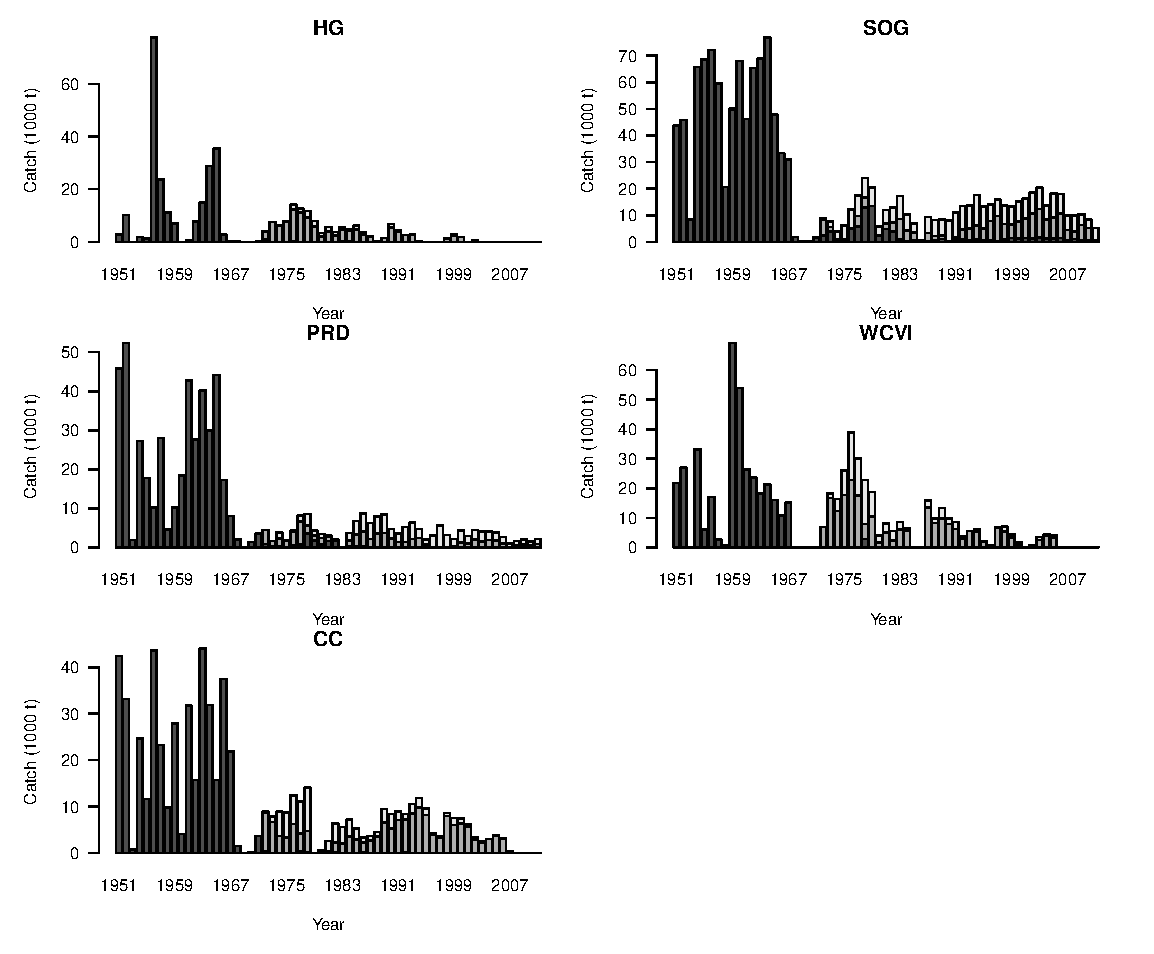
\includegraphics[width=\textwidth]{../Figs/iscam_fig_CatchMajorAreas.pdf}\\
	\caption{Historical catch of herring in the five major stock areas between 1951 and 2011 for the winter purse seine fishery (dark bars), seine-roe fishery (grey bars), and gillnet fishery (light grey bars). Units of catch are in thousands of metric tons.}\label{FigCatch}
\end{figure}
	
	\subsubsection{Relative abundance data}
Herring spawn surveys have been conducted throughout the B.C. coast beginning in the 1930s. Prior to 1988, spawn surveys were conducted from the surface either by walking the beach at low tide or using a drag from a skiff to estimate the shoreline length and width of spawn. Egg layers were sampled visually and are used to calculate egg densities following the methods of \cite{schweigert2001stock}. Beginning in 1988, herring spawn surveys using SCUBA methods were introduced and were implemented coastwide within a couple of years initially being conducted by DFO staff and eventually through contract divers hired through the test fishing program. Prior to the 2006 Larocque ruling, the test fishing program was funded through an allocation of fish by industry. In years since the 2006 Larocque ruling, the availability of resources to conduct dive surveys in all areas has been reduced. For 2011, dive surveys were conducted in all major and minor assessment regions, with the exception of Area 2W where snorkelling and surface survey methods were also used. As in earlier years, a few minor spawning beds outside the main assessment areas were surveyed by SCUBA or surface methods where resources permitted.


The locations of the spawning beds for the five major and two minor stock areas are shown in Figure \ref{figSpawnMaps}.  Egg density estimates are used to calculate a fishery-independent index of herring spawning biomass, referred to as the spawn survey index hereafter \citep{schweigert2001stock}.

\begin{figure}[!tbp]
	% Requires \usepackage{graphicx}
	\centering
	\includegraphics[scale=0.35]{../Figs/PBSfigs/2011_spawn_HG_2E_July13.pdf}
	\includegraphics[scale=0.35]{../Figs/PBSfigs/2011_spawn_HG_2W_July13.pdf}\\
	\includegraphics[scale=0.35]{../Figs/PBSfigs/2011_spawn_PRD_July13.pdf}
	\caption{Preliminary Spawning activity for Haida Gwaii (top panels) and Prince Rupert District (bottom) in 2011.}
\end{figure}
\begin{figure}[!tbp]
	% Requires \usepackage{graphicx}
	\ContinuedFloat
	\centering
	\includegraphics[scale=0.35]{../Figs/PBSfigs/2011_spawn_CCJuly13.pdf}
	%\includegraphics[scale=0.5]{../Figs/PBSfigs/2011-SOG-Prelim-WG.pdf}
	\includegraphics[scale=0.35]{../Figs/PBSfigs/2011_spawn_SOG_July13.pdf}\\
	\includegraphics[scale=0.35]{../Figs/PBSfigs/2011_spawn_WCVI_August16.pdf}
	\caption{Preliminary Spawning activity for Central Coast (top left panel), Strait of Georgia (top right) in 2011 and west coast Vancouver Island (bottom).}\label{figSpawnMaps}
\end{figure}
% \begin{figure}[!tbp]
% 	% Requires \usepackage{graphicx}
% 	\ContinuedFloat
% 	\centering
% 	%\includegraphics[scale=0.5]{../Figs/PBSfigs/2011-WCVI-Prelim-WG.pdf}\\
% 	\includegraphics[scale=0.5]{../Figs/PBSfigs/2011_spawn_WCVI_August16.pdf}\\
% 	\caption{Preliminary Spawning activity in 2011 for the West Coast of Vancouver Island (includes minor stock area 27).}\label{figSpawnMaps}
% \end{figure}

	The spawn survey is conducted after the fisheries in the area have been completed; therefore, it is assumed that all the mortality for the year has occurred just prior to commencing the spawning survey. The fisheries independent survey estimates egg density and total spawn area, and from this information the total female spawning biomass can be estimated assuming the 200 eggs per gram of female  or 100 eggs per gram of mature  individuals \citep{hay1985reproductive,hardwick1973biomass}. The assumed selectivity for the spawn survey is fixed to the maturity schedule for herring.  	
	
\begin{figure}[!tbp]
	% Requires \usepackage{graphicx}
	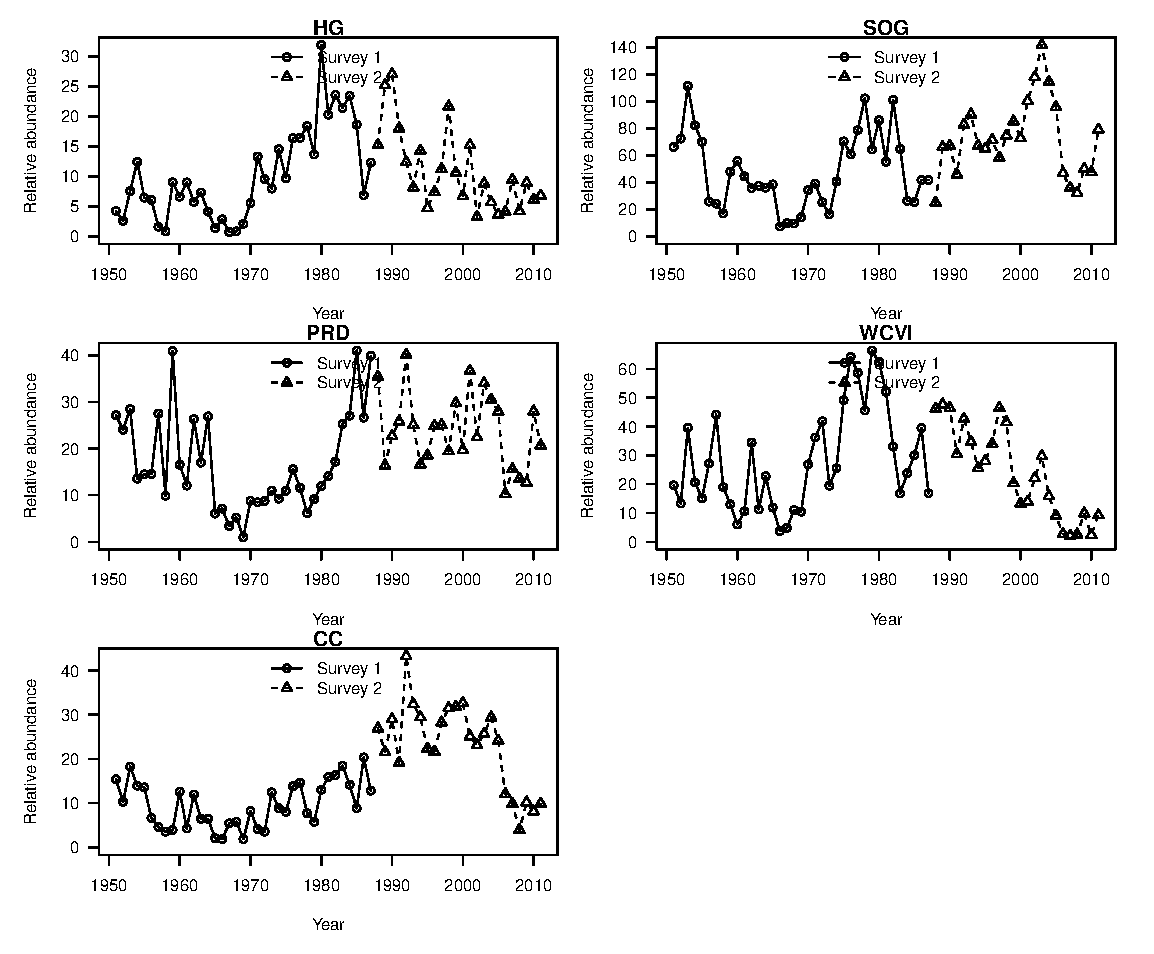
\includegraphics[width=\textwidth]{../Figs/iscam_fig_SurveyMajorAreas.pdf}\\
	\caption{Spawn survey index for Strait of Georgia between 1951 and 2011. The units are actual estimates of spawning biomass (1000s tons), but only the trend information is used in the model fitting.}\label{FigSurvey}
\end{figure}
	
	\subsubsection{Biological samples}
	
	Biological samples are collected from both commercial catch and from the test fishery program.  Commencing  in 1975, test fishery charters supplemented biological samples in areas with poor sampling that was not representative of the stock in that area (i.e., fishing solely on spawning aggregations), or in closed areas. Prior to 2006, test fishing charters were funded through an allocation of fish to the test program; the program is now fully funded by DFO.  Through a contract with DFO, the Herring Conservation and Research Society (HCRS) sub-contracts a number of vessels to collect biological samples.  Industry also conducts pre-season test sets for roe-quality testing in open areas and supplementary biological samples are provided as part of this program.  The following data are collected for all biological samples: fish length, weight, sex, and maturity.  Subsequently these sources of data are combined and information on weight-at-age and proportion-at-age become input data for the stock assessment model.
	
	During the 2010/2011 season a total of 248 biological samples were collected, of which 151 were collected from the test fishery, 57 were collected from the roe fishery, 16 from the food \& bait fishery, 4 from Spawn on Kelp (SOK) operations, and 16 from the summer trawl research survey (Table \ref{table:PartII:bioSamples}).  Note that the definition of a sample is roughly 100 individual fish.  A summary of biological samples collected from commercial and pre-fishery charters from 2002/03--2010/11 is presented in Table \ref{table:PartII:sampleSizes}).

\begin{table}
	\caption{Summary of biological samples collected and processed from all sources from the 2010/11 herring season.}
	\label{table:PartII:bioSamples}
	\begin{center}
		\begin{tabular}{cccccc}
		\hline
		& \multicolumn{3}{c}{Commercial samples} &  \\
		Stock & Roe fishery & SOK fishery & F\&B & Test fishery & Research\\
		\hline
		HG (QCI 2E) &  &  &  & 13\\
		PRD & 29 & 1 &  & 24\\
		CC &  &  &  & 30\\
		SOG & 18 &  & 20 & 60\\
		WCVI &  &  &  & 14 & 16\\
		Area 2W &  &  &  & 10\\
		Area 27 &  & 3\\
		Other Areas\\
		\hline
		Total & 57 & 4 & 16 & 151 & 16\\
		\hline
		\end{tabular}
	\end{center}
\end{table}

\begin{table}
	\caption{Summary of biological samples collected and processed from commercial catch and test fishery charters from 2002/03-2010/11.}
	\label{table:PartII:sampleSizes}
	\begin{center}
\begin{tabular}{cccc}
\hline
Fishing season & Commercial fishery samples & Charter and research samples & Total\\
\hline
2002/03 & 120 & 287 & 407\\
2003/04 & 79 & 222 & 301\\
2004/052 & 83 & 191 & 274\\
2005/06 & 46 & 164 & 210\\
2006/07 & 114 & 85 & 199\\
2007/08 & 116 & 103 & 219\\
2008/09 & 87 & 136 & 223\\
2009/10 & 78 & 135 & 213\\
2010/11 & 81 & 167 & 248\\
\hline
\end{tabular}
	
	\end{center}
\end{table}
	
	
	
	%%Insert Summary of biological samples from the 2010/2011 season here:
	
	%%Insert Summary of biological samples collected and processeed from commercial catch etc. here (Table 2 from Cleary 2011).
	
	\subsubsection{Age composition data}
	
	Ageing data, through the reading of fish scales, are collected from the biological samples taken from the commercial fisheries and test fishery charters. Age composition data is used to determine proportions-at-age and is an essential source of input data to the herring stock assessment model.
	
	Catch-at-age data from the winter seine fishery (top panels of Figures \ref{FigAgeCompsHG}-\ref{FigAgeCompsWCVI}) tend to consist of younger fish in comparison to the age composition data from the seine-roe and gillnet fleets post 1970. The shaded polygons in Figures \ref{FigAgeCompsHG}-\ref{FigAgeCompsWCVI} approximates the 95\% distribution of ages in the catch.  Roughly 90\% of the fish landed in the winter seine fishery were younger than age-7, and younger than age-6 in recent years.  In both the winter seine and seine-roe fishery age-2 fish are frequently landed; whereas, age-2 fish are rarely landed in the gillnet fishery, and fish do not appear to fully recruit to the gear until at least 4-5 years of age.  The mean age of the catch appears to be increasing between 2008 and 2010 in both the gillnet and winter seine fishery, and there is no obvious trend in the seine roe fishery.  There is however a declining trend in the older ages caught in the seine-roe fishery since 2006 (erosion of age-structure).

\begin{sidewaysfigure}[!tbp]
	% Requires \usepackage{graphicx}
	\centering
	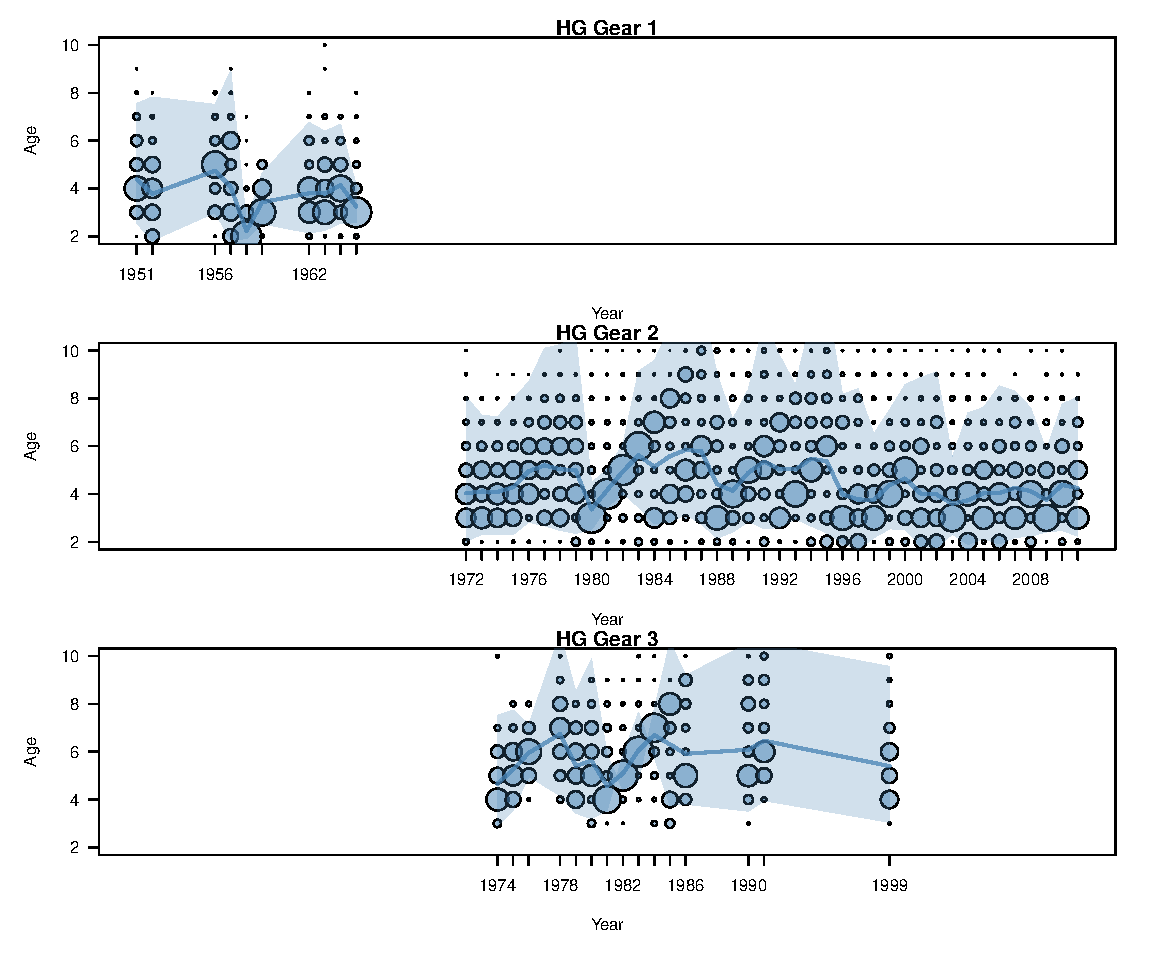
\includegraphics[width=0.85\textwidth]{../Figs/iscam_fig_AgeCompsHG.pdf}\\
	\caption{Bubble plots showing the proportions-at-age versus time for the winter purse seine fishery (top), seine roe fishery (middle) and the gillnet fishery (bottom) in Haida Gwaii.  The area of the circle is proportional to cohort abundance, each column sums to 1, zeros are not shown, and age 10 is a plus group. Also shown is the mean age of the catch (line) and the approximate 95\% distribution of ages (shaded polygon) for each year.}\label{FigAgeCompsHG}
\end{sidewaysfigure}

\begin{sidewaysfigure}[!tbp]
	% Requires \usepackage{graphicx}
	\centering
	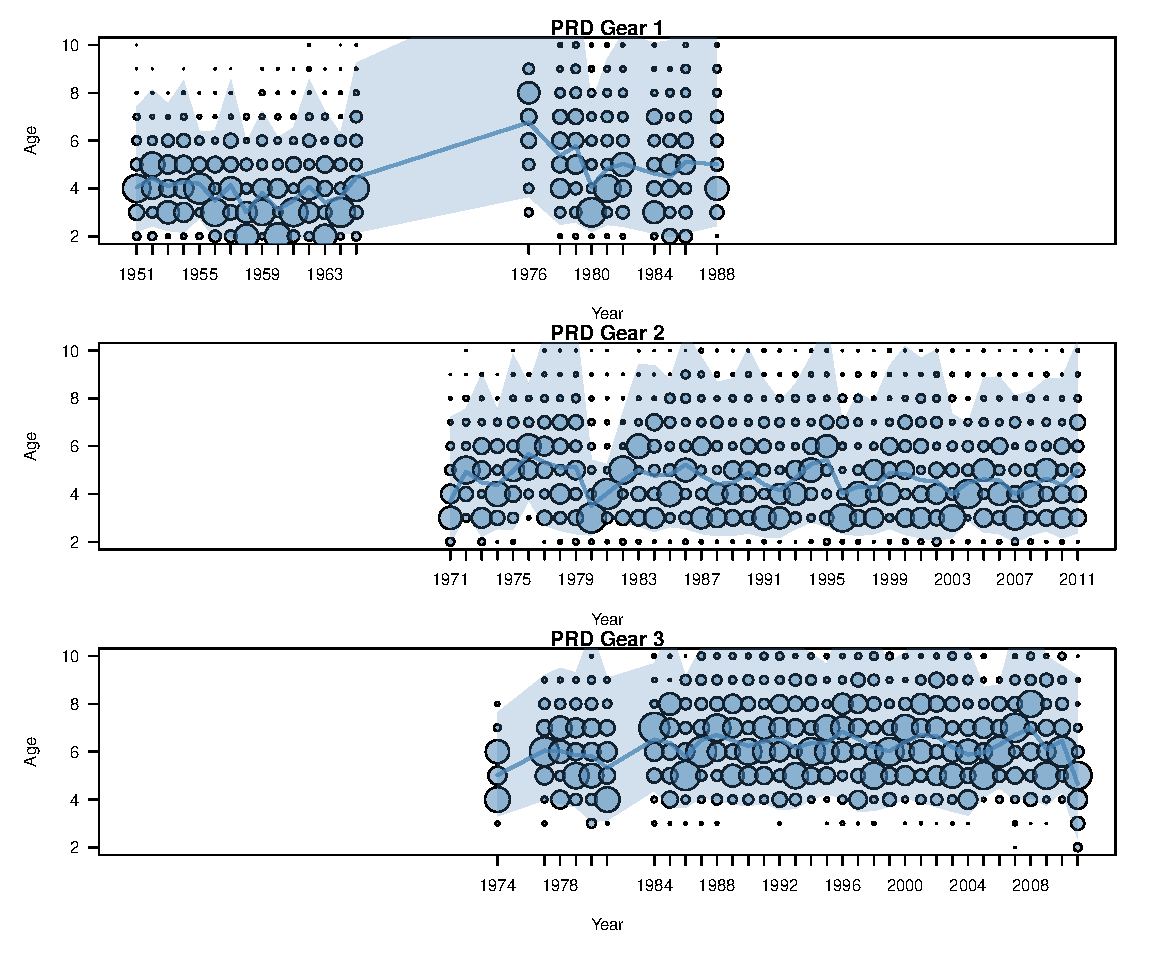
\includegraphics[width=0.85\textwidth]{../Figs/iscam_fig_AgeCompsPRD.pdf}\\
	\caption{Bubble plots showing the proportions-at-age versus time for the winter purse seine fishery (top), seine roe fishery (middle) and the gillnet fishery (bottom) in Prince Rupert District.  The area of the circle is proportional to cohort abundance, each column sums to 1, zeros are not shown, and age 10 is a plus group. Also shown is the mean age of the catch (line) and the approximate 95\% distribution of ages (shaded polygon) for each year.}\label{FigAgeCompsPRD}
\end{sidewaysfigure}

\begin{sidewaysfigure}[!tbp]
	% Requires \usepackage{graphicx}
	\centering
	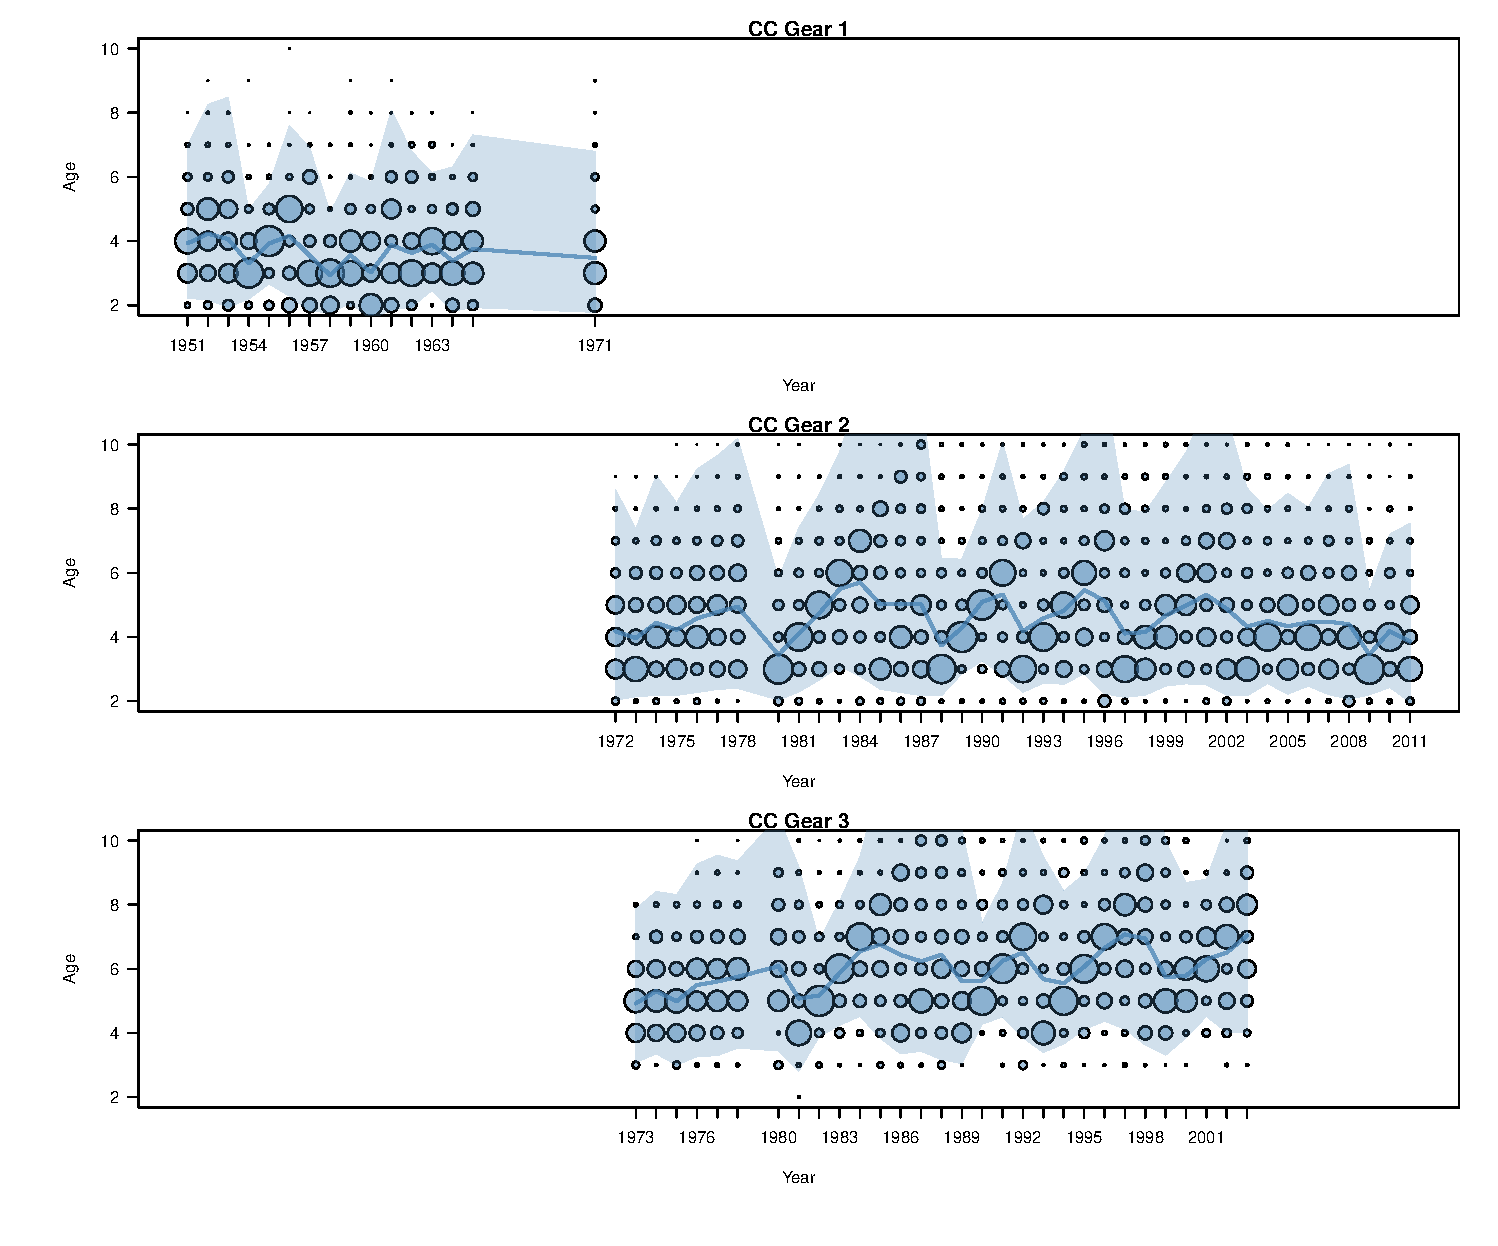
\includegraphics[width=0.85\textwidth]{../Figs/iscam_fig_AgeCompsCC.pdf}\\
	\caption{Bubble plots showing the proportions-at-age versus time for the winter purse seine fishery (top), seine roe fishery (middle) and the gillnet fishery (bottom) in the Central Coast region.  The area of the circle is proportional to cohort abundance, each column sums to 1, zeros are not shown, and age 10 is a plus group. Also shown is the mean age of the catch (line) and the approximate 95\% distribution of ages (shaded polygon) for each year.}\label{FigAgeCompsCC}
\end{sidewaysfigure}

\begin{sidewaysfigure}[!tbp]
	% Requires \usepackage{graphicx}
	\centering
	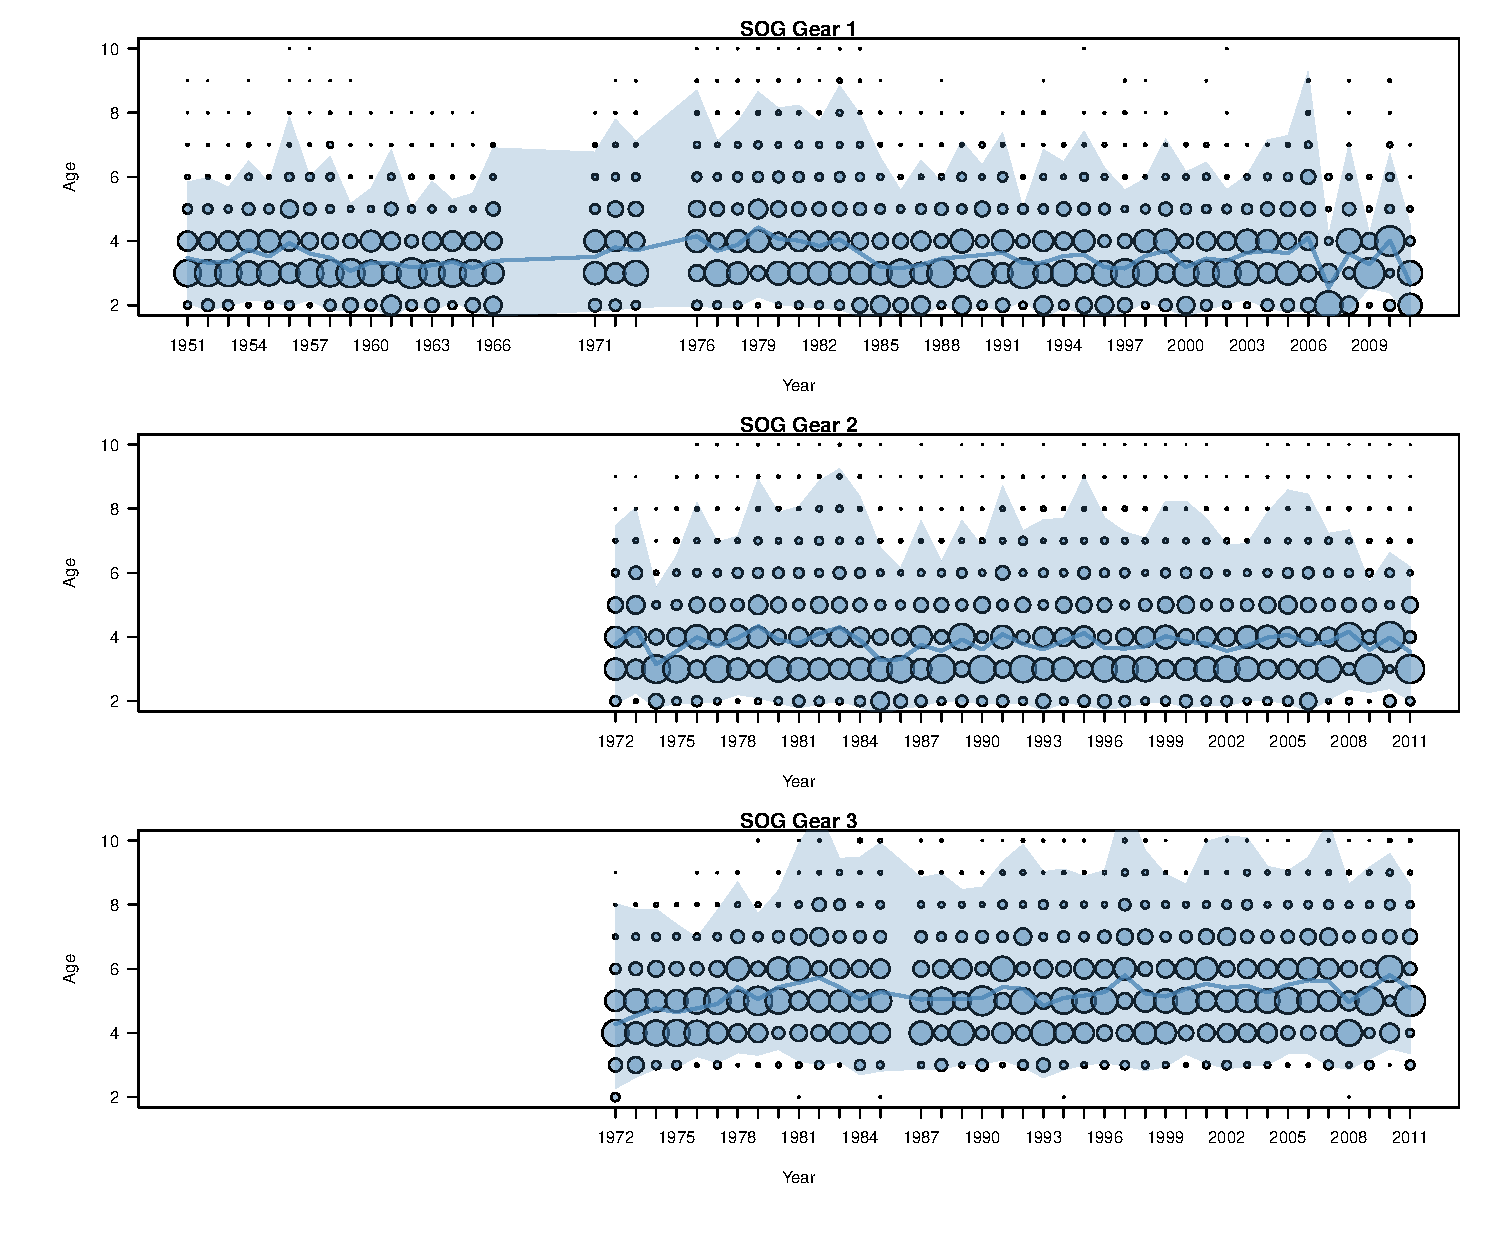
\includegraphics[width=0.85\textwidth]{../Figs/iscam_fig_AgeCompsSOG.pdf}\\
	\caption{Bubble plots showing the proportions-at-age versus time for the winter purse seine fishery (top), seine roe fishery (middle) and the gillnet fishery (bottom) in the Strait of Georgia.  The area of the circle is proportional to cohort abundance, each column sums to 1, zeros are not shown, and age 10 is a plus group. Also shown is the mean age of the catch (line) and the approximate 95\% distribution of ages (shaded polygon) for each year.}\label{FigAgeCompsSOG}
\end{sidewaysfigure}

\begin{sidewaysfigure}[!tbp]
	% Requires \usepackage{graphicx}
	\centering
	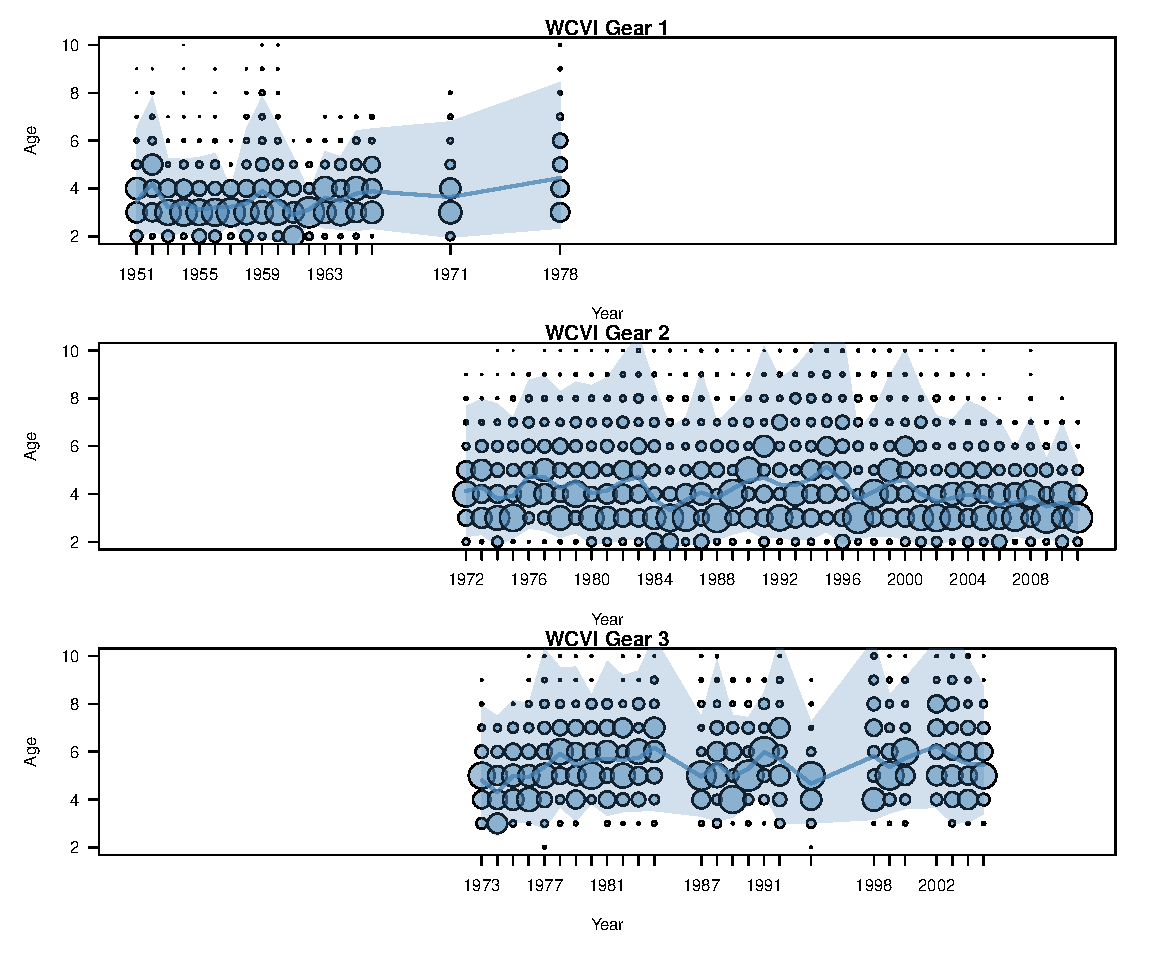
\includegraphics[width=0.85\textwidth]{../Figs/iscam_fig_AgeCompsWCVI.pdf}\\
	\caption{Bubble plots showing the proportions-at-age versus time for the winter purse seine fishery (top), seine roe fishery (middle) and the gillnet fishery (bottom) in the West Coast Vancouver Island region.  The area of the circle is proportional to cohort abundance, each column sums to 1, zeros are not shown, and age 10 is a plus group. Also shown is the mean age of the catch (line) and the approximate 95\% distribution of ages (shaded polygon) for each year.}\label{FigAgeCompsWCVI}
\end{sidewaysfigure}





	\subsubsection{Mean weight-at-age data}

	From the mid-1970s until the present, there has been a measurable decline in weight-at-age for all ages in all major stock areas (Figure \ref{FigMeanWt}). Samples collected during the 2009/10 fishing year indicate weights-at-age that are among the lowest on record. This declining weight-at-age may be attributed to any number of factors, including: fishing effects (i.e., gear selectivity), environmental effects (changes in ocean productivity), or it may even be attributed to changes in sampling protocols (shorter time frame over which samples are collected). Declining weight-at-age has been observed in all five of the major stocks, and despite area closures over the last 10-years, has continued to occur in the QCI and WCVI stocks. Although the direct cause of this decline is still to be investigated, this trend has been observed in B.C. and U.S. waters, from California to Alaska \citep{schweigert2002herring}, and merits further research.	The observed mean weight-at-age data appear to have a few  errors that need to be investigated as well; for example, see the apparently small age-10 fish in 2001 in Figure \ref{FigMeanWt}.

\begin{figure}[!tbp]
	% Requires \usepackage{graphicx}
	\centering
	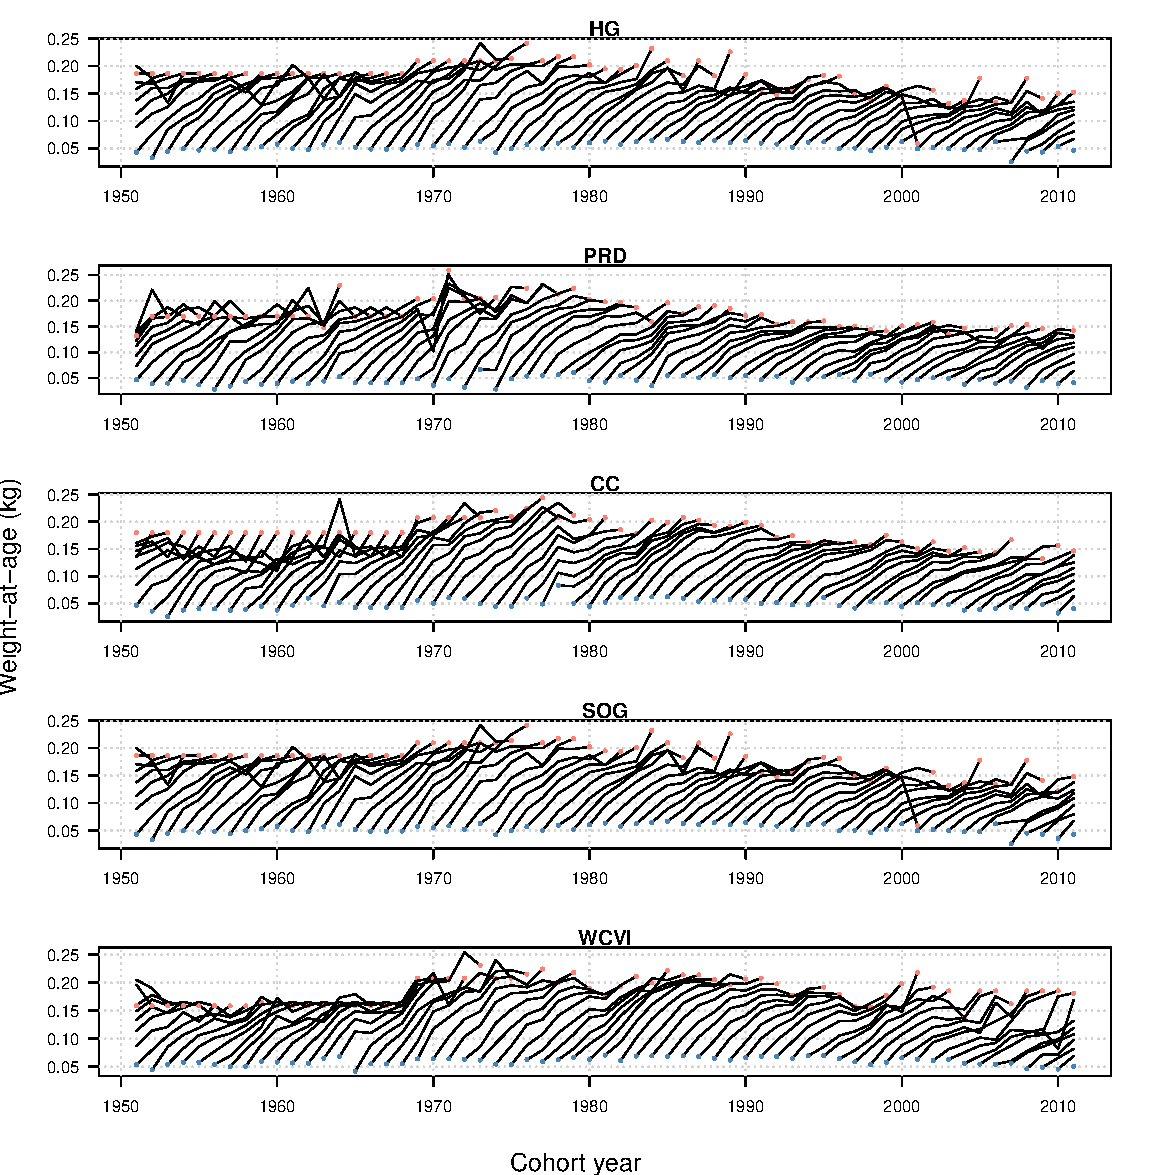
\includegraphics[width=\textwidth]{../Figs/iscam_fig_MeanWt.pdf}\\
	\caption{Empirical mean weight-at-age data by cohort from 1951 to 2011 for ages 2 to 10 in the five major Stock Assessment Regions.}\label{FigMeanWt}
\end{figure}
	

%%%%%%%%%%%%%%%%%%%%%%%%%%%%%%%%%%%%%%%%%%%%%%%%%%%%%%%%%%%%%%%%%%%%%
%%%%%%%%%%%%%%%%%%%%%%%%%%%%%%%%%%%%%%%%%%%%%%%%%%%%%%%%%%%%%%%%%%%%%
%%%%%%%%%%%%%%%%%%%%%%%%%%%%%%%%%%%%%%%%%%%%%%%%%%%%%%%%%%%%%%%%%%%%%	
	\subsection{Analytical methods}

	For the 2011 BC herring assessment, \iscam was used to conduct the stock assessment for each of the five major Stock Assessment Regions (SAR) and two minor assessment areas (Area 2W and Area 27).  The technical details of this model can be found in Appendix \ref{appiSCAM}.
		
	\subsection{Retrospective analysis}
	A retrospective analysis was conducted for each of the major and minor SARs.  The retrospective analysis successively removes the last 10-years of data and examines changes in estimates of terminal spawning biomass.  The results are then plotted on a single panel to compare how estimates of spawning biomass change as successive years of data are omitted from the analysis.
	
	\subsection{Abundance and recruitment forecasts}
	The abundance forecast for the upcoming fishing season, also referred to as pre-fishery biomass, is defined as the predicted biomass of age-4 fish and older plus the number of age-3 fish recruiting in year $T+1$.  The abundance estimates are based on the median values from the sampled posterior distribution.  Age-3 recruits are based on poor, average, and good recruitment scenarios; see next paragraph for definitions of poor, average and good.
	
	The recruitment forecasts are based on the surviving number of age-3 fish at the start of the fishing season times the average weight-at-age 3 in the last 5 years. The definitions of poor, average, and good recruitment are as follows: \textbf{Poor} is the average recruitment from the 0-33 percentile, \textbf{Average} is the average recruitment from the 33-66 percentile, and \textbf{Good} is the average recruitment from the 66-100 percentile.  Note that all cohorts from 1951 to 2011  were included in the calculation of recruitment quantiles.
	
	\subsection{Catch advice}
Catch advice is based on the application of the harvest control rule (HCR). The herring HCR has three components:
\begin{enumerate}
\item Reference points (LRP, USR, and cuttoffs)
\item Harvest rate
\item Decision rules
\end{enumerate}

For each of the five major stocks, the limit reference point (LRP) is the cuttoff value, which is defined here as 0.25\bo\, and the	Upper Stock Reference (USR) is defined as the 1.05*LRP (0.25\bo\ + 0.2*0.25\bo = LRP + 0.05LRP). \textbf{For clarification, references to \bo\ throughout this document refer to the mature spawning stock biomass.} The default harvest rate if the stock is at or above USR is 0.2, and declines linearly to 0 when the stock is at or below the LRP (a default harvest rate of 0.1 is used for the minor stock areas).  The decision rule for the major stock areas operates as follows:

\begin{itemize}
	\item If the forecast run is less than the LRP (cuttoff) then the area is closed to all commercial harvest  (i.e., stock is deemed to be in the critical zone).
	
	\item If the forecast run is greater than the LRP and less than the USR (i.e., cautious zone), then total allowable catch is based on a reduced harvest rate that would deplete the stock to the LRP level.
	
	\item If the forecast run is greater than USR, then the total allowable catch is set at 20\% of the forecast run.
\end{itemize}



	

%!TEX root=../Selex.tex
% Statisitcal fit

% Retrospective performance.

% Estimated reference points.

\section*{Results} % (fold)
\label{sec:results}

\subsection*{Statisical fit} % (fold)
\label{sub:statisical_fit}

Statisitics summarizing how well each model fits a single realization of simulated data are based on the overall objective function value, Deviance Information Criterion (DIC) and the Root Mean Square Error (RMSE) between observed and predicted quantities (Table \ref{tab:statisticalPeformance}). Under conditions in which the true selectivity is fixed (scenmario 1), similar fits to the relative survey abundance index and age-composition data (see Survey RMSE and Survey age RMSE in Table \ref{tab:statisticalPeformance}) were obtained  irrespective of the form of the assumed selectivity curve for the commercial fishery.  However, fits to the commercial age-composition data markedly improved under the time-varying age-based selectivity model (c).  Allowing for additional structure in the selectivity coefficients over time resulted in decreases in the RMSE from 0.48, 0.41 and 0.33 for models (a), (b), and (c), respectively for the commercial age-composition information (Table \ref{tab:statisticalPeformance}).  The worst fit to the commercial age-composition was obtained for the bicubic spline model (d).

We do not recommend basing model selection solely on statistical criterion, such as DIC, but for statistical comparison we provide DIC and $\Delta$DIC values to give a sense of the relative differences between the various assessment models for each simulation case.  In the cases examined here (Table \ref{tab:statisticalPeformance}), DIC always favors the most structurally complex model (c) with the largest number of estimated selectivity parameters. The large improvement in fit for model (c) is always due to explaining more residual variation in the age-composition data. All other models appear to fit the survey index and age-composition equally, regardless if the data were generated from fixed selectivities or complex time-varying selectivities.  This is not an unexpected result, as the observation models for the survey age composition data are structurally consistent with the simulation model.  What is significant is that the use of the conditional maximum likelihood estimate of the variance to weight the commercial age-composition data is down-weighted when the incorrect selectivity model is specified for the commercial selectivities. However, it should be noted that this down-weighting incorrectly assigns process error to observation error due to mis-specification of selectivity.




\begin{table*}[!tbh]
	\caption{Statistical performance based on the objective function value, effective number of estimated parameters, DIC, $\Delta$DIC, Root Mean Square Error (RMSE) in recruitment deviations, survey abundance residuals, and the age-composition residuals for models fit to fixed, discrete time blocks and continous changes in commercial selectivity.}
	\label{tab:statisticalPeformance}
	\begin{center}
		\begin{tabular}{l|cccc}
		\hline

		\hline
		\textbf{} & \textbf{Fixed (a)} & \textbf{Discrete (b)} & \textbf{Continuous (c)} & \textbf{Bicubic spline (d)} \\
		\hline

		
	    \multicolumn{5}{l}{\textbf{\underline{True selectivity is fixed}}}\\
		Objective function            &  -836.41 &  -918.16 & -1208.16 &  -939.17 \\
		Eff. No. parameters             &    96 &   116 &   334 &   173 \\
		DIC              & -1479.77 & -1601.51 & -1739.09 & -1528.01 \\
		$\Delta$DIC         &   259.32 &   137.58 &     0.00 &   211.08 \\
		Recruitment RMSE &     1.04 &     1.04 &     1.06 &     1.04 \\
		Survey RMSE      &     0.25 &     0.25 &     0.26 &     0.26 \\
		Commercial RMSE         &     0.47 &     0.40 &     0.32 &     0.49 \\
		Survey age RMSE         &     0.24 &     0.25 &     0.25 &     0.24 \\
		%Total.RMSE       &     2.03 &     1.96 &     1.90 &     2.06 \\
		
		\hline
		\multicolumn{5}{l}{\textbf{\underline{True selectivity has 3 time blocks}}}\\
		Objective function            &  -775.49 & -1051.57 & -1335.82 & -1028.80 \\
		Eff. No. parameters             &    96 &   116 &   337 &   173 \\
		DIC              & -1356.24 & -1868.57 & -1990.44 & -1707.88 \\
		$\Delta$DIC         &   634.20 &   121.87 &     0.00 &   282.56 \\
		Recruitment RMSE &     1.04 &     1.04 &     1.05 &     1.05 \\
		Survey RMSE      &     0.26 &     0.26 &     0.26 &     0.26 \\
		Commercial RMSE         &     0.52 &     0.35 &     0.29 &     0.45 \\
		Survey age RMSE         &     0.25 &     0.29 &     0.25 &     0.24 \\
		%Total.RMSE       &     2.10 &     1.92 &     1.86 &     2.02 \\

		\hline
		\multicolumn{5}{l}{\textbf{\underline{True selectivity changes annually}}}\\
		Objective function            &  -717.56 &  -788.52 & -1029.41 &  -785.91 \\
		Eff. No. parameters             &    96 &   116 &   333 &   173 \\
		DIC              & -1241.22 & -1342.26 & -1382.43 & -1222.14 \\
		$\Delta$DIC         &   141.21 &    40.17 &     0.00 &   160.29 \\
		Recruitment RMSE &     1.06 &     1.09 &     1.12 &     1.05 \\
		Survey RMSE      &     0.26 &     0.26 &     0.27 &     0.26 \\
		Commercial RMSE         &     0.52 &     0.44 &     0.35 &     0.56 \\
		Survey age RMSE         &     0.27 &     0.29 &     0.30 &     0.27 \\
		%Total.RMSE       &     2.14 &     2.10 &     2.07 &     2.17 \\



		% Objective function  & -1452.78 &  -1461.06 &  -1695.12 &  -1538.09 \\
		% Eff. No. parameters &    96    &    110    &    344    &    175    \\
		% DIC                 & -2712.84 &  -2701.20 &  -2696.89 &  -2723.12 \\
		% $\Delta$DIC         &    10.28  &    21.92 &     26.23 &      0.00 \\
		% Recruitment RMSE    &     1.03 &      1.03 &      1.03 &      1.03 \\
		% Survey RMSE         &     0.25 &      0.26 &      0.25 &      0.25 \\
		% Commercial RMSE     &     0.28 &      0.28 &      0.20 &      0.26 \\
		% Survey age RMSE     &     0.26 &      0.26 &      0.27 &      0.26 \\

		
		% \hline
		% Objective function  & -1340.49 &  -1428.81 &  -1689.57 &  -1516.78 \\
		% Eff. No. parameters &    96    &    109    &    345    &    175    \\
		% DIC                 & -2487.96 &  -2638.03 &  -2683.48 &  -2680.78 \\
		% $\Delta$DIC         &   195.52 &     45.45 &      0.00 &      2.70 \\
		% Recruitment RMSE    &     1.04 &      1.04 &      1.03 &      1.03 \\
		% Survey RMSE         &     0.25 &      0.26 &      0.25 &      0.25 \\
		% Commercial RMSE     &     0.32 &      0.29 &      0.20 &      0.26 \\
		% Survey age RMSE     &     0.26 &      0.26 &      0.27 &      0.26 \\

		
		% \hline
		% Objective function  & -1293.30 &  -1304.14 &  -1543.59 &  -1376.39 \\
		% Eff. No. parameters &    95    &    109    &    344    &    177    \\
		% DIC                 & -2394.61 &  -2387.88 &  -2393.28 &  -2396.33 \\
		% $\Delta$DIC         &     1.72 &      8.45 &      3.05 &      0.00 \\
		% Recruitment RMSE    &     1.13 &      1.13 &      1.12 &      1.12 \\
		% Survey RMSE         &     0.26 &      0.27 &      0.27 &      0.27 \\
		% Commercial RMSE     &     0.30 &      0.30 &      0.21 &      0.28 \\
		% Survey age RMSE     &     0.33 &      0.34 &      0.33 &      0.32 \\

		\hline

		\hline
		\end{tabular}
	\end{center}
\end{table*}
The effective number of estimated parameters is based on the difference between the expectation of the deviance and the deviance based on the expectation of the parameter values.  The larger the effective number of parameters is a measure of how well the model fits the data.  In all cases the effective number of parameters was equal to or greater than the number of parameters estimated in the model.  In the case of model (c) the effective number of parameters ($\approx$335) is much greater than the 319 that were actually estimated in the ADMB code.  However, it should also be noted that the variance parameters for age-composition residuals and the scaling parameter $q$ \citep[see][]{walters1994calculation} are based on the conditional maximum likelihood estimates, rather than explicitly estimating them inside the model code.  This parameterization implies an additional 67 parameters and hence the effective number of parameters is much less than the 386 parameters in model (c).  Again, we caution the use of DIC for model selection in cases where data are weighted via conditional maximum likelihood estimate of the variance.


% For the cases where the true selectivity is based on a fixed logistic function, the most appropriate model based on DIC is model (d) where a bicubic spline is used to model selectivity. The RMSE terms for model (d) are less than the true underlying values that were used to generate the data, which is of no surprice when additional flexibility in selectivity can accomodate some of the residual variance in age-composition in the form of minor changes in selectivity (Table \ref{tab:statisticalPeformance}).   This pattern of explaining the residual variation is virtually the same regardless of what the true underlying selectivity pattern is.

% In the case where the true selectivity changes discretely over three time blocks, assessment models with time-varying selectivity (c) and (d) appear to fit the data better that models that assumed fixed selectivity (a), or even the discrete changes in selectivity (see $\Delta$DIC values in Table \ref{tab:statisticalPeformance}).  For this particular case, it's better to allow for continous changes in selectivity than to 
% assume fixed values.

% In the case where the true selectivity changes annually, based on relative cohort abundance, the model results were a bit more surprising.  The expectation would be that assuming fixed selectivity would perform less well than allowing for time-varying selectivity.  Based on the $\Delta$DIC values obtained in Table \ref{tab:statisticalPeformance} there is very little differnce between models that allow for continous changes in selectivity (models c and d) and fixed selectivity (model a).  There was less weight for the model that allows for discrete-block changes in selectivity (model b).

% Similar results were also obtained in the case where true selectivity changes annually (as a function of the relative cohort abundance).  However, the difference between assuming block selectivity and fixed selectivity resulted in negligble differences in the $\Delta$AIC values.  Moreover, the RMSE for the age-composition data was greater than the true values used to generate the observation errors in age-sampling in models (a) and (b). For model (c), the RMSE was less than the true value for the commercial age-composition, and  in model (d) it was identical to the true value.   

% subsection statisical_fit (end)
\subsection*{Retrospective performance} % (fold)
\label{sub:retrospective_performance}

Two useful graphical tools for examining retrospective problems in stock assessment models are referred to here as spaghetti plots (Fig. \ref{fig:retrospectiveSSB}), and squid plots (Fig. \ref{fig:retrosquidbase}), respectively.  In the spaghetti plots, successive estimates of spawning stock biomass based on sequentially removing the terminal year of data for four previous years are overlayed on each panel.  In addition to the estimated spawning biomass in Fig. \ref{fig:retrospectiveSSB}, the true spawning biomass that was used to generate simulated data is also shown for reference.  In the squid plots, successive estimates of spawning biomass relative to the  spawning biomass in the terminal year of data are overlaid.  In Fig. \ref{fig:retrosquidbase}, the percent bias is shown as the relative difference between the true values; hence a 100\% bias implies that the stock size is over-estimated by a factor of 2.  


\begin{figure*}[!tbh]
	\begin{center}
		\includegraphics[angle=0,width=\textwidth]{./FIGS/fig:RetroSpectiveSSB.png}
	\end{center}
	\caption{One realization of retrospective estimates of spawning biomass for simulated Pacific hake populations where four years of data was sequentially removed from.  The true spawning biomass used to simulated the data is included for reference.}
	\label{fig:retrospectiveSSB}
\end{figure*}

Based on the maximum likelihood results from a single realization shown in Fig. \ref{fig:retrospectiveSSB}, there is a tendency for the model to systematically over-estimate the spawning stock biomass in the terminal years.  This trend is largely a function of the recent downward trend in abundance since the mid 2000s, and not a persistent feature of the stock assessment model.  In the case of the true selectivity being fixed over time, the least amount of retrospective bias occurred in the simple models (a) and (b), and the largest bias was observed for model (c).  Similar results were also obtained in the discrete changes in selectivity (row 2 of Fig. \ref{fig:retrosquidbase}) as well as the time-varying changes in selectivity.  Also of interest is the retrospective behavior in model (d) where the sequential removal of the terminal year data results in changing the knot positions in the bicubic spline (see early years on column (d) of Fig. \ref{fig:retrosquidbase}). Retrospective  estimates of spawning biomass earlier in the time series of model (d) are slightly more variable in comparison to models with fixed selectivities (a), (b), and even in the case where selectivity is allowed to vary annually (c).  However, these results are from a single realization, and should not be used to make general inferences in retrospective bias.  Median values from a series of Monte Carlo trials would be more appropriate for making general inferences.  These results from a single realization merely illustrate that despite additional structural flexibility associated with time-varying selectivity, large retrospective bias can still occur. 



% For the simulated data based on fixed selectivity, the qualitative pattern in retrospective bias was similar for all four alternative selectivity scenarios (Figure \ref{fig:retrospectiveSSB}, 1a, ..., 1d).   The worst performing models were the cases with continuous changes in selectivity over time (1c and 1d), with maximum estimates of retrospective bias relative to the terminal values approaching 25\% for the bicubic spline model (Figure \ref{fig:retrosquidbase}).  

% For cases based on simulated data with discrete time blocks in selectivity, the least amount of bias was observed in the case where the correct model was specified (Figure \ref{fig:retrosquidbase}, 2b).  Assuming fixed selectivity or continuous changes in selectivity resulted in significantly more retrospecitve bias.  Assuming fixed selectivity also resulted in further departures from the true spawning biomass in the initial years.

\begin{figure*}[!tbh]
	\begin{center}
		\includegraphics[angle=0,width=\textwidth]{./FIGS/fig:RetroSquidBase.png}
	\end{center}
	\caption{One realization of retrospective estimates of bias in spawning biomass relative to spawning biomass estimated with all available data.  These biases are based on the same spawning biomass trajectories in Figure \ref{fig:retrospectiveSSB}.}
	\label{fig:retrosquidbase}
\end{figure*}


% \begin{figure}[tb]
% 	\begin{center}
% 		\includegraphics[angle=90,width=0.85\textwidth]{../FIGS/fig:RetroSquid.png}
% 	\end{center}
% 	\caption{Retrospective estimates of bias in spawning biomass relative to the true spawning biomass used to simulated the data.  These biases are based on the same spawning biomass trajectories in Figure \ref{fig:retrospectiveSSB}.}
% 	\label{fig:retrosquid}
% \end{figure}

% In the cases where the true selectivity varies over time, the retrospective performance was least biased for the models that assume time-varying selectivity (Figure \ref{fig:retrosquidbase}, 3c and 3d).  Retrospective peformance is much worse if the selectivity is assumed to be constant, or change in a series of blocks, when the real underlying process is continuous change in selectivity (Figure \ref{fig:retrosquid}, 3a and 3b). 

% Monte Carlo retrospective results. Make general statement that less retrospective bias when assuming more structural complexity.  May be better to assume a penalized random walk in selectivity than to not.

Over a number of Monte Carlo trials (40 independent data sets) the patterns in retrospective bias over the alternative selectivity assumptions differ from the single realization shown in Fig. \ref{fig:retrospectiveSSB}.  To quantify retrospective bias, a series of summary statistics were used to measure the trade-off between precision and bias in the retrospective analyses (Table \ref{tab:RetroStatistics}).  The mean bias $\mu$ reflects the average difference between the terminal and retrospective year spawning biomass and is generally lowest for models that allow for time-varying selectivity (models (c) and (d) in Table \ref{tab:RetroStatistics}).  The absolute mean bias $|\mu|$ better characterizes the mean retrospective  variation.  For example, in model 3c (Table \ref{tab:RetroStatistics}) the mean bias $\mu$ is relatively small, but the mean absolute difference over four retrospective years is very large.  This is also reflected in the summary statistic $\Omega$ and the Mean Absolute Deviation (MAD).  Even though model 3c is the correct model for the simulations with continuous changes in selectivity, the results in Table \ref{tab:RetroStatistics} suggest that model 3d would be preferable due to less mean bias and a lower overall variance in the potential bias.  

\begin{table*}[!tbh]
	\caption{Retrospective bias statistics for each model run, where $\mu_1$ corresponds to the mean bias over four retrospective years, $\mu_2$ is the absolute mean, $\Omega$ is a combined measure of mean and absolute bias, and MAD is the Mean Absolute Deviation of $\mu_2$.  Lower MAD scores imply less variability in retrospective bias estimates.}
	\label{tab:RetroStatistics}
	\begin{center}
	\begin{footnotesize}
		
		\begin{tabular}{l|cccc|cccc|cccc}
		\hline

		\hline
		&\multicolumn{4}{c|}{\textbf{Fixed}} & \multicolumn{4}{c|}{\textbf{Discrete}} & \multicolumn{4}{c}{\textbf{Continous}} \\
		&\textbf{1a}  &\textbf{1b}  &\textbf{1c}  &\textbf{1d}  &\textbf{2a}   &\textbf{2b}  &\textbf{2c}  &\textbf{2d}  &\textbf{3a}  &\textbf{3b}  &\textbf{3c}  &\textbf{3d}\\
		\hline
		$\mu_1$     &-9.14& -8.26& -1.55& -1.77& -8.88& -12.57& -1.11& -3.11& -6.72& -5.90& -2.09& -0.83\\
		$\mu_2$ &14.19& 13.63& 13.46& 12.78& 12.94&  14.96& 12.12& 13.75& 14.06& 14.08& 17.99& 13.85\\
		$\Omega$  &19.13& 18.28& 17.49& 16.53& 17.58&  20.66& 15.73& 17.86& 18.62& 18.47& 22.97& 18.08\\
		MAD    & 4.77&  4.68&  6.42&  4.93&  5.32&   6.28&  5.11&  5.48&  4.73&  4.84& 10.51&  5.78\\

		\hline

		\hline
		\end{tabular}
	\end{footnotesize}
	\end{center}
\end{table*}

Similar results were also obtained for the simulations involving fixed selectivities and discrete time blocks with less overall mean bias, and lower MAD's, for models with continuous changes in selectivity over time (Table \ref{tab:RetroStatistics}).


% subsection retrospective_performance (end)


\subsection*{Estimated reference points} % (fold)
\label{sub:estimated_reference_points}


The impacts of model specification on the estimates of MSY-based reference points are summarized using a series of box-plots (Fig. \ref{fig:RefPointBias}) based on Monte Carlo trials.  In each box plot the $\ln$ ratios of the estimated versus true values are shown where the median bias is based on the solid bar.  In the case where the true model is based on fixed selectivity, estimated reference points are relatively unbiased ($\pm$ 10\%); however, the precision of the estimates decreases with increasing model complexity (Fig. \ref{fig:RefPointBias}).  There is a bit of a trend in the estimate of $F_{\rm{MSY}}$ that corresponds to an increase in overall stock productivity with assumed increases in model complexity.  This same increasing trend is also present, but less pronounced, in the estimates of MSY.  These trends indicate that the overall scale and productivity of the estimated population increases with increasing model complexity. 

In cases where the true model is based on scenario 2, estimated $F_{\rm{MSY}}$ reference points were biased upwards for model (a)  because the true selectivity shifts towards smaller fish later in the time series (Fig. \ref{fig:RefPointBias}). The vast majority of the age-composition data were based on selectivities curves that target larger fish and the constant selectivity assumption in model (a) does not capture this trend. Estimates of MSY were less biased in this case. Estimates of spawning biomass reference points ($B_{\rm{MSY}}$ and $B_o$) were less sensitive to the assumed model structure, with the exception of model (a) being fit to scenario 2. Recall that the MSY-based reference points are based on selectivity values in the terminal year. Under the assumption of constant selectivity, estimates of $F_{\rm{MSY}}$ are almost certain to be biased with the rare exception that the terminal year selectivity corresponds to the estimated average selectivity.  

\begin{figure*}[!tbh]
	\begin{center}
		\includegraphics[width=\textwidth]{./FIGS/fig:RefPointBias.png}
	\end{center}
	\caption{Estimates of precision and bias for fishing mortality rate reference points ($F_{\rm{MSY}}$), maximum sustainable yield (MSY), spawning biomass as MSY ($B_{\rm{MSY}}$) and the unfished spawning biomass ($B_o$) based on Monte Carlo trials using data simulated from fixed, discrete blocks and continuous changes in selectivity. }
	\label{fig:RefPointBias}
\end{figure*}

For the case where the true model involves continuous changes in selectivity, or scenario 3, estimates of $F_{\rm{MSY}}$ for all models are biased upwards (Fig. \ref{fig:RefPointBias}).  Estimates of $F_{\rm{MSY}}$ are more variable for models that have a large number of estimated selectivity parameters, indicating that estimates of selectivity in the terminal year are highly imprecise (recall that MSY-based reference points were based on estimated selectivity in the terminal year). All other reference points are much less biased if a more complex assessment model is assumed in comparison to the underlying simulation model.


% RMSE resultz
In all of the Monte Carlo simulation-estimation experiments the variance components for recruitment deviations, survey index errors, age-composition data for both the commercial and survey samples were estimated.  The root mean square error (RMSE) of the residuals is a proximate measure of how each of the data series are weighted internally in the assessment model.   The distribution of the RMSE values for each error component is shown in Fig. \ref{fig:RMSEdist} for scenarios 1-3 using models (a)-(d).  The RMSE values for the survey abundance index for all scenario and model combinations were very similar to the true standard deviation of 0.3 that was used to generate the simulated observation errors (Fig. \ref{fig:RMSEdist}).   For scenarios (1) and (2), the RMSE value for the recruitment deviations were also similar to the true standard deviation of $\sigma_R=1.12$ in the simulated recruitment deviations.  For scenario (3) however, RMSE values were greater than 1.12 under the assumption that selectivity changes annually  as in model (c), but less so under model (d) where changes selectivity is constrained via the bicubic spline interpolation.

\begin{figure*}[!tbh]
	\begin{center}
		\includegraphics[width=\textwidth]{./FIGS/fig:RMSEdist.png}
	\end{center}
	\caption{Distribution of Root Mean Squared Error values for the recruitment deviations, survey residuals, commercial and survey age-composition residuals based on 40 Monte Carlo trials.}
	\label{fig:RMSEdist}
\end{figure*}

The pattern of RMSE values for the commercial age composition samples generally decreases with increasing flexibility in the selectivity model (Fig. \ref{fig:RMSEdist}, lower left panel), with the exception of the bicubic spline model.  The simulated size-based selectivities in all of the model scenarios was very dynamic owing to the large changes in the empirical size-at-age data in Pacific hake (Fig. \ref{fig:simSelex}). The bicubic spline model used in model (d) estimates a total of 60 knots (7 for age, and 12 for years), and interpolates over age, not size-at-age.  In this case, the bicubic spline performs rather poorly in comparison to fixed size-based selectivities and the annual age-based selectivity due to the tension imposed by the limited number of knots.

Another pattern in the distributions of RMSE values shown in Fig. \ref{fig:RMSEdist} that is of significant interest is how the weight of the survey age-composition data changes with changes in assessment models.  In scenario 1 and 2, the distribution of RMSE values is fairly similar for all assessment models, and here we note that the variability in RMSE values increases with increasing number of estimated selectivity coefficients.  However, in scenario (3) with continuous changes in commercial selectivity being the true case, the relative RMSE values increase (i.e., poorer fit) for the survey age-composition data.  In other words, more structurally complex assessment models fit the commercial age-composition better at the partial expense of putting less weight on the survey age-composition.  But note that the RMSE values for 3c are roughly equal to the true standard deviation of $\sigma_2=0.3$ in the multivariate logistic sampling distribution.  

For model (d), relatively poor fits were obtained for the commercial age-composition data, and RMSE values for this model were much larger than model (c).  However, model (d) fit the survey age-composition data better and does not allow for increased process errors in the form of recruitment deviations in comparison to model (c).  In short, annual changes in selectivity greatly improves the fit to commercial age-composition data, but this comes at the expense of poorer fits to the survey age-composition data and increased recruitment variation. 


% The distribution of the RMSE values from the Monte Carlo trials displayed pretty consistent patters over each alternative dataset (Figure \ref{fig:RMSEdist}).  The residual fit to the survey abundance index was very similar across all simulated datasets and all alternative assessment models.  The true coefficient of variation used in simulating the true data was fixed at 0.3, and accounting for the bias correction in the lognormal errors, the theoretical RMSE in the residuals should be approximately 0.255.  The standard deviation in the simulated recruitment residuals was fixed at 1.12 and the distribution of RMSE values is very similar for the fixed selectivity and time-block selectivity simulated datasets (Figure \ref{fig:RMSEdist}).  In the case where the simulated data was based on continouse changes in selectivity, the RMSE values for the recruitment deviations was slightly higher than the true value, presumably to allow for more variation in recruitment that could be explained by annual changes in selectivity.

% The pattern of RMSE values for the commercial age-composition residuals was consistent across simulated datasets, where largest RMSE values were always observed with fixed selectivity (Figure \ref{fig:RMSEdist}, model a), and the smallest under the annual time-varying selectivity (Figure \ref{fig:RMSEdist}, model c).  Models with intermediate complexity were able to explain more residual variation in the comercial age-composition(models b and d, respectively).  

% subsection estimated_reference_points (end)

\subsection*{Simulation performance} % (fold)
\label{sub:simulation_performance}




To qualitatively evaluate how each of the four alternative selectivity models would perform if the analyst was na\"ive about the underlying true selectivity, we use a simple rank order system (Table \ref{tab:rankorder}).  For example, if DIC was the statistical basis for choosing the most appropriate selectivity model then based on the simulation results in Table \ref{tab:statisticalPeformance} when the true underlying model is based on fixed selectivity, the rank order of DIC values (low to high) is model c, b, d, and a. If the underlying model is not known, the DIC criterion favors model (c) the most, and model (d) the second most.    Based on all of the criterion listed in Table \ref{tab:rankorder}, the most appropriate model to choose if in fact the analyst was na\"ive about the underlying processes in selectivity would be model (c).    Model (b) also ranks fairly high; however, this assumes the correct block time-periods can be identified from residual analysis or historical knowledge of fishing practices.

\begin{table*}[!tbh]
	\caption{Ranking of model based on Deviance Information Criterion, RMSE, retrospective bias and bias in the estimates of $F_{\rm{MSY}}$ and MSY based on Monte Carlo trials. Each column ranks the assumed selectivity model from most likely (left) to least likely (right) for simulation case study.  The top-two ranks represent the most and second most frequently selected model.}
	\label{tab:rankorder}
	\begin{center}
		\begin{tabular}{l|ccc|c}
		\hline

		\hline
		\textbf{Criterion} & \textbf{Fixed} & \textbf{Discrete} &\textbf{Continuous} & \textbf{Top-two ranks} \\
		\hline
		DIC from Tab. \ref{tab:statisticalPeformance}
		           & c,b,d,a & c,b,d,a & c,b,d,a & c,b\\
		\hline
		Retrospective    & d,c,a,b & c,d,a,b & d,a,b,c & c,d\\
		$F_{\rm{MSY}}$   & b,c,a,d & c,d,b,a & c,b,a,d & c,b\\
		MSY              & d,c,b,a & c,d,b,a & d,a,c,b & d,c\\
		RMSE             & c,b,a,d & c,b,a,d & c,b,a,d & c,b\\
		% RMSE           & c,d,a,b & c,d,b,a & c,d,a,b & c,d\\
		% Retrospective  & d,b,a,c & d,a,c,b & a,b,d,c & d,b\\
		% $F_{\rm{MSY}}$ & c,d,a,b & c,d,a,b & a,b,d,c & c,d\\
		\hline

		\hline
		\end{tabular}
	\end{center}
\end{table*}

% subsection simulation_performance (end)

% section results (end)
%!TEX root=../Selex.tex
\section*{Discussion} % (fold)
\label{sec:discussion}

% Summary of the study
The over-arching objective of this simulation study was to determine if it is safe to assume more structural complexity in selectivity when in fact the real data come from a simple stationary process, and is it safer to assume simple structural complexity when real data come from a fishery with dynamic changes in selectivity.  To address this objective, a simulation model based with length-based selectivity and variable length-at-age by year was used to generate simulated data for four alternative assessment models that assumed: (a) selectivity was length-based and stationary, (b) selectivity was length-based and changed discretely in four time periods, and (c) selectivity was age-based and allowed to change each year, and (d) selectivity was age-based and interpolated over age and year using a bicubic spline and 60 equally spaced knots.  From the perspective of a n\"iave analyst who is unfamiliar with the history of the fishery and data, it may infact be safer to adopt a penalized likelihood approach to incorporate time-varying selectivity.


A more appropriate approach to specific case studies would be to develop a closed-loop feedback control system and an appropriate loss function to better elucidate which selectivity parameterization is more appropriate for achieving intended management objectives.  This is also known in the fisheries realm as management strategy evaluation \cite{MSE Crowds}.  Having an appropriate loss function to judge the performance of each alternative model would greatly improve model selection criterion from a policy performance perspective.

% section discussion (end)

\part{Effects of reduced minimum-size limits on yield, spawning biomass, and wastage.}
\setcounter{chapter}{2}
\setcounter{section}{0}
cutoff%!TEX root = /Users/stevenmartell/Documents/CURRENT PROJECTS/iSCAM-trunk/fba/BC-herring-2011/WRITEUP/BCHerring2011.tex


\section{Introduction}

The objectives of this section of the report are: (1) present the data used in the 2011 assessment, (2) provide a summary overview of the integrated statistical catch-age model (hereafter, \iscam), (3) present the 2011 stock assessment and forecast for 2012, and (4) describe in detail the decision table used to provide advice to fisheries management.

BC herring are currently managed as five major stocks and 2 minor stocks (Figure \ref{Fig1}).  Annual catch advice for each of these areas is based on current estimates of stock status, and a 20\% exploitation rate if the post-fishery stock is above the cutoff level for the five major stocks and a 10\% exploitation rate for the two minor stocks.  Cutoff levels for the five major stocks historically were based on the 1996 estimate of  0.25$B_o$.  These cutoffs are currently thought to be more conservative 	than the suggested default Limit Reference Point of 0.4\bmsy\ \citep{dfo2006}. For example, \bmsy\ is normally in the range of 35\% of the unfished biomass for many fish stocks; therefore,  40\% of \bmsy is roughly 14\% of  unfished which is significantly lower than the 25\%$B_o$ that is currently used for Pacific herring.   Alternative cutoffs based on updated estimates of $B_o$ are also provided in this document.

This years assessment is based on a new model, \iscam, where alternative assumptions about survey $q$, and the form of the error distribution for the age-composition data are the major differences in comparison to the 2010 assessment using HCAM.  In addition to the changes in likelihoods, we also present an alternative parametrization of the gillnet selectivity to determine if the residual variation in gillnet age-composition data are better explained by systematic changes in the empirical weight-at-age data or selectivity has been relatively constant and natural mortality rates have varied over time.


In this part of the document, we first describe the five major and two minor Stock Assessment Regions (SARS) that comprise the BC herring stocks. We then present the input data used in this years assessment, briefly describe the analytical methods and diagnostics, describe the recruitment and catch forecasts, and the Harvest Control Rule (HCR) used for generating catch advice. We then present the maximum likelihood estimates of residual patterns and overall fits to the observations, summarize MSY based reference points and maximum likelihood estimates of \bo. Lastly, we present the results of integrating the joint posterior distribution, diagnostics for ensuring convergence, marginal parameter distributions (with prior distributions overlaid), and catch advice based on the median values of the joint posterior distribution.  The last section presents the data, MLE results, marginal distributions and catch advice for the two minor areas (the HCR in the minor area differs from the major areas).


\section{BC Herring Stocks}
The geographic boundaries used to delineate the B.C. herring stock assessment regions have remained consistent since 1993.  Boundaries and locations of the major stock and minor stock areas are identified in Figure \ref{Fig1}.  The Haida Gwaii (HG) or Queen Charlotte Islands (QCI2E) stock assessment region includes most of Statistical Area 2E, spanning from Cumshewa Inlet in the north to Louscoone Inlet in the south.  The Prince Rupert District (PRD) stock assessment region encompasses Statistical Areas 03 to 05.  The Central Coast (CC) assessment region separates the major migratory stocks from the minor spawning populations in the mainland inlets.  The Central Coast assessment region includes Statistical Area 07 plus Kitasu Bay in Area 06, Kwakshua Channel in Section 085 and Fitz Hugh Sound in Section 086.  The Strait of Georgia (SOG) stock assessment region includes all of Statistical Areas 14 to 19, 28, and 29 (excluding Section 293), Deepwater Bay and Okisollo Channel, both in Section 132, and Section 135.  The west coast of Vancouver Island (WCVI) assessment region encompasses Statistical Areas 23 to 25.  The minor stocks include all of Area 27 and Area 2W (excluding Louscoone Inlet in Section 006).  Current geographic stock boundaries are outlined in \cite{Midgley:2003fk}, although note that SOG sections 280 and 291 do not appear as they were added in 2006.

%%\begin{figure}[!tbp]
%%	% Requires \usepackage{graphicx}
%%	%\includegraphics[width=\textwidth]{Figs/HerringAreaMap.pdf}
%%	\includegraphics[width=0.95\textwidth]{../FIGS/PBSfigs/Assessment_Regions_2W_27_2010_HG.pdf}
%%	\caption{B.C. herring major stock areas: Haida Gwaii (HG or QCI 2E), Prince Rupert District (PRD), Central
%%Coast (CC), Strait of Georgia (SOG), West Coast Vancouver Island (WCVI), and minor stock areas: Area 2W and
%%Area 27.}\label{II:fig:map}
%%\end{figure}
%!TEX root = /Users/stevenmartell/Documents/CURRENT PROJECTS/iSCAM-trunk/fba/BC-herring-2011/WRITEUP/BCHerring2011.tex
\section{Methods}
	\subsection{Input data \& assumptions}
	\subsubsection{Catch data}
	For each of the statistical areas, the required input data for \iscam\ consists of a catch time series for each of the fishing fleets.  For the BC herring fishery, the annual total removals has been partitioned into three distinct fishing fleets (or fishing periods, see Figure \ref{FigCatch}).  The first fleet is a winter seine fishery that has been in operation since the start of the assessment in 1951, the second is a seine-roe fishery that commenced in 1972 in the Strait of Georgia, and the third fleet is a gillnet fishery that targets females on the spawning grounds. The model is fit to the catch time series information and assumes measurement errors are lognormal, independent and identically distributed.  The assumed standard deviation in the catch observations must be specified in the control file and it is assumed that measurement errors in the catch is the same for all fishing periods.  The units of the catch are given in 1000s of metric tons.
	
	In addition to the commercial catch, removals from fisheries independent surveys must also be specified in \iscam. Two additional fleets are specified to represent the spawn survey, where the spawn survey is broken into two distinct time periods pre-1988 and post-1988, the year when the survey switched from surface surveys to dive surveys.  This partitioning of the data is done for two reasons: (1) to allow for different catchability coefficients to be specified for the early and late periods, and to allow for more weight to be placed on the contemporary data due to improved precision in the estimates of egg layers. 

%TODO decide if the test fishery data is going to be looked at here or in the appendix
	In the case where the test fishery data has been separated from the seine roe fishery, an additional fleet is specified in the data file and fishing mortality rates for the test fishery are also estimated in years when the catch is greater than 0.
	
\begin{figure}[!tbp]
	% Requires \usepackage{graphicx}
	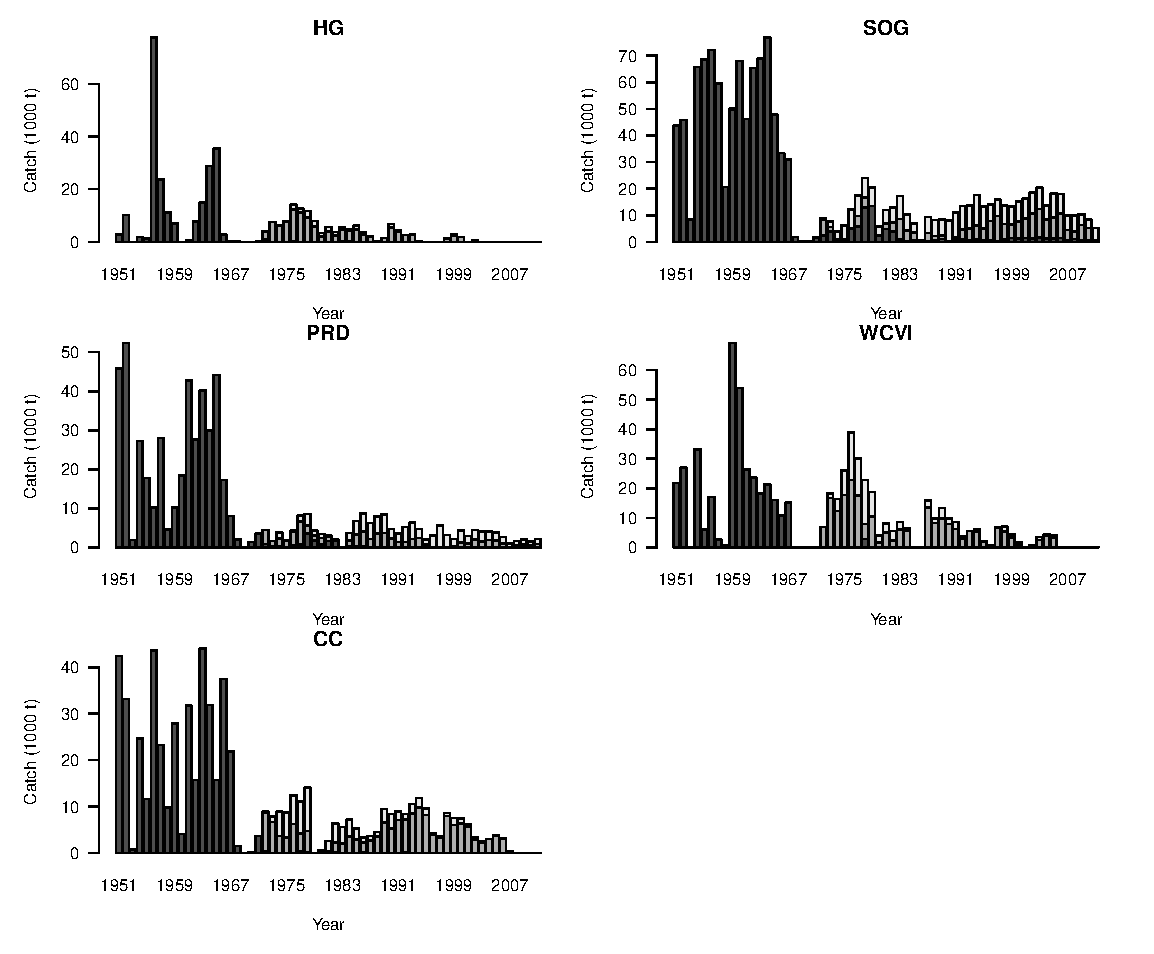
\includegraphics[width=\textwidth]{../Figs/iscam_fig_CatchMajorAreas.pdf}\\
	\caption{Historical catch of herring in the five major stock areas between 1951 and 2011 for the winter purse seine fishery (dark bars), seine-roe fishery (grey bars), and gillnet fishery (light grey bars). Units of catch are in thousands of metric tons.}\label{FigCatch}
\end{figure}
	
	\subsubsection{Relative abundance data}
Herring spawn surveys have been conducted throughout the B.C. coast beginning in the 1930s. Prior to 1988, spawn surveys were conducted from the surface either by walking the beach at low tide or using a drag from a skiff to estimate the shoreline length and width of spawn. Egg layers were sampled visually and are used to calculate egg densities following the methods of \cite{schweigert2001stock}. Beginning in 1988, herring spawn surveys using SCUBA methods were introduced and were implemented coastwide within a couple of years initially being conducted by DFO staff and eventually through contract divers hired through the test fishing program. Prior to the 2006 Larocque ruling, the test fishing program was funded through an allocation of fish by industry. In years since the 2006 Larocque ruling, the availability of resources to conduct dive surveys in all areas has been reduced. For 2011, dive surveys were conducted in all major and minor assessment regions, with the exception of Area 2W where snorkelling and surface survey methods were also used. As in earlier years, a few minor spawning beds outside the main assessment areas were surveyed by SCUBA or surface methods where resources permitted.


The locations of the spawning beds for the five major and two minor stock areas are shown in Figure \ref{figSpawnMaps}.  Egg density estimates are used to calculate a fishery-independent index of herring spawning biomass, referred to as the spawn survey index hereafter \citep{schweigert2001stock}.

\begin{figure}[!tbp]
	% Requires \usepackage{graphicx}
	\centering
	\includegraphics[scale=0.35]{../Figs/PBSfigs/2011_spawn_HG_2E_July13.pdf}
	\includegraphics[scale=0.35]{../Figs/PBSfigs/2011_spawn_HG_2W_July13.pdf}\\
	\includegraphics[scale=0.35]{../Figs/PBSfigs/2011_spawn_PRD_July13.pdf}
	\caption{Preliminary Spawning activity for Haida Gwaii (top panels) and Prince Rupert District (bottom) in 2011.}
\end{figure}
\begin{figure}[!tbp]
	% Requires \usepackage{graphicx}
	\ContinuedFloat
	\centering
	\includegraphics[scale=0.35]{../Figs/PBSfigs/2011_spawn_CCJuly13.pdf}
	%\includegraphics[scale=0.5]{../Figs/PBSfigs/2011-SOG-Prelim-WG.pdf}
	\includegraphics[scale=0.35]{../Figs/PBSfigs/2011_spawn_SOG_July13.pdf}\\
	\includegraphics[scale=0.35]{../Figs/PBSfigs/2011_spawn_WCVI_August16.pdf}
	\caption{Preliminary Spawning activity for Central Coast (top left panel), Strait of Georgia (top right) in 2011 and west coast Vancouver Island (bottom).}\label{figSpawnMaps}
\end{figure}
% \begin{figure}[!tbp]
% 	% Requires \usepackage{graphicx}
% 	\ContinuedFloat
% 	\centering
% 	%\includegraphics[scale=0.5]{../Figs/PBSfigs/2011-WCVI-Prelim-WG.pdf}\\
% 	\includegraphics[scale=0.5]{../Figs/PBSfigs/2011_spawn_WCVI_August16.pdf}\\
% 	\caption{Preliminary Spawning activity in 2011 for the West Coast of Vancouver Island (includes minor stock area 27).}\label{figSpawnMaps}
% \end{figure}

	The spawn survey is conducted after the fisheries in the area have been completed; therefore, it is assumed that all the mortality for the year has occurred just prior to commencing the spawning survey. The fisheries independent survey estimates egg density and total spawn area, and from this information the total female spawning biomass can be estimated assuming the 200 eggs per gram of female  or 100 eggs per gram of mature  individuals \citep{hay1985reproductive,hardwick1973biomass}. The assumed selectivity for the spawn survey is fixed to the maturity schedule for herring.  	
	
\begin{figure}[!tbp]
	% Requires \usepackage{graphicx}
	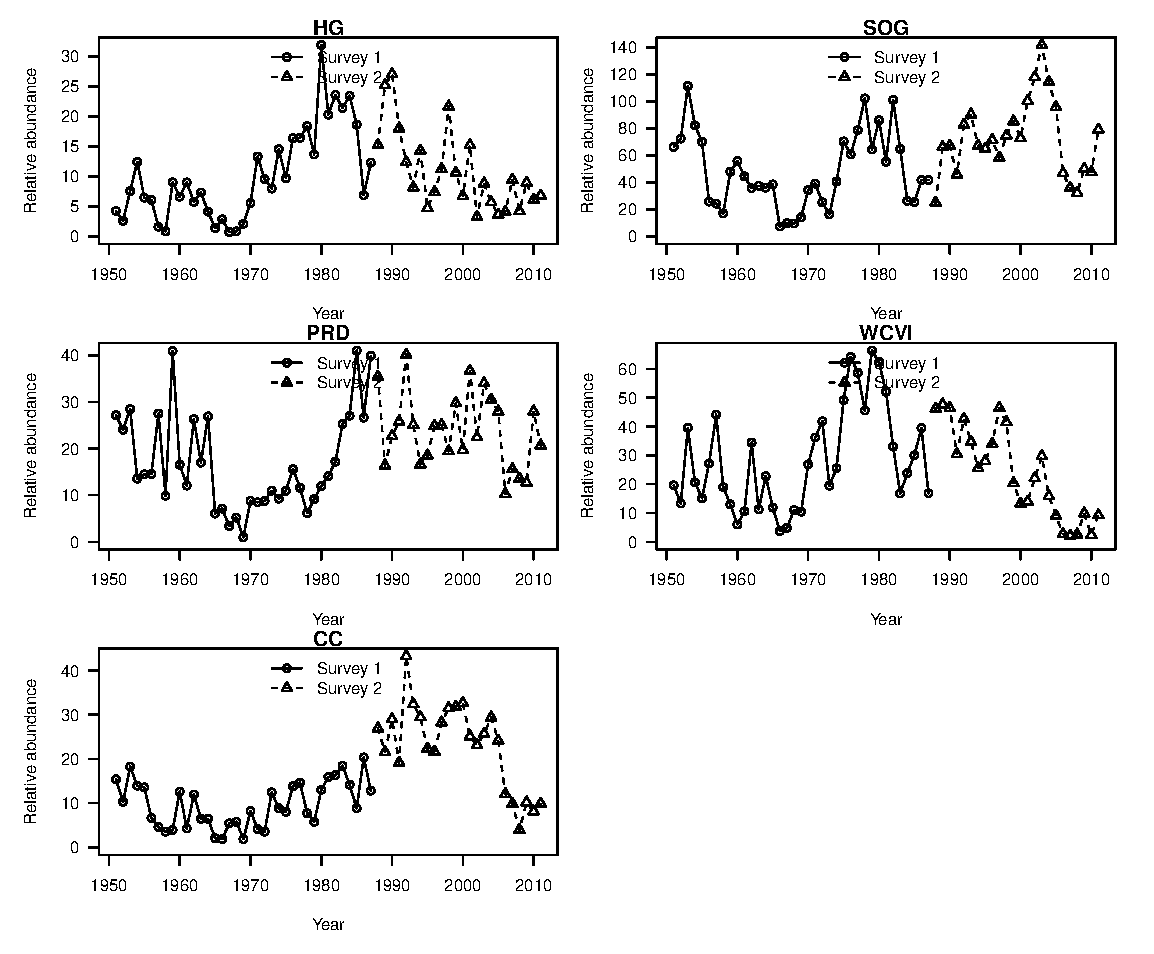
\includegraphics[width=\textwidth]{../Figs/iscam_fig_SurveyMajorAreas.pdf}\\
	\caption{Spawn survey index for Strait of Georgia between 1951 and 2011. The units are actual estimates of spawning biomass (1000s tons), but only the trend information is used in the model fitting.}\label{FigSurvey}
\end{figure}
	
	\subsubsection{Biological samples}
	
	Biological samples are collected from both commercial catch and from the test fishery program.  Commencing  in 1975, test fishery charters supplemented biological samples in areas with poor sampling that was not representative of the stock in that area (i.e., fishing solely on spawning aggregations), or in closed areas. Prior to 2006, test fishing charters were funded through an allocation of fish to the test program; the program is now fully funded by DFO.  Through a contract with DFO, the Herring Conservation and Research Society (HCRS) sub-contracts a number of vessels to collect biological samples.  Industry also conducts pre-season test sets for roe-quality testing in open areas and supplementary biological samples are provided as part of this program.  The following data are collected for all biological samples: fish length, weight, sex, and maturity.  Subsequently these sources of data are combined and information on weight-at-age and proportion-at-age become input data for the stock assessment model.
	
	During the 2010/2011 season a total of 248 biological samples were collected, of which 151 were collected from the test fishery, 57 were collected from the roe fishery, 16 from the food \& bait fishery, 4 from Spawn on Kelp (SOK) operations, and 16 from the summer trawl research survey (Table \ref{table:PartII:bioSamples}).  Note that the definition of a sample is roughly 100 individual fish.  A summary of biological samples collected from commercial and pre-fishery charters from 2002/03--2010/11 is presented in Table \ref{table:PartII:sampleSizes}).

\begin{table}
	\caption{Summary of biological samples collected and processed from all sources from the 2010/11 herring season.}
	\label{table:PartII:bioSamples}
	\begin{center}
		\begin{tabular}{cccccc}
		\hline
		& \multicolumn{3}{c}{Commercial samples} &  \\
		Stock & Roe fishery & SOK fishery & F\&B & Test fishery & Research\\
		\hline
		HG (QCI 2E) &  &  &  & 13\\
		PRD & 29 & 1 &  & 24\\
		CC &  &  &  & 30\\
		SOG & 18 &  & 20 & 60\\
		WCVI &  &  &  & 14 & 16\\
		Area 2W &  &  &  & 10\\
		Area 27 &  & 3\\
		Other Areas\\
		\hline
		Total & 57 & 4 & 16 & 151 & 16\\
		\hline
		\end{tabular}
	\end{center}
\end{table}

\begin{table}
	\caption{Summary of biological samples collected and processed from commercial catch and test fishery charters from 2002/03-2010/11.}
	\label{table:PartII:sampleSizes}
	\begin{center}
\begin{tabular}{cccc}
\hline
Fishing season & Commercial fishery samples & Charter and research samples & Total\\
\hline
2002/03 & 120 & 287 & 407\\
2003/04 & 79 & 222 & 301\\
2004/052 & 83 & 191 & 274\\
2005/06 & 46 & 164 & 210\\
2006/07 & 114 & 85 & 199\\
2007/08 & 116 & 103 & 219\\
2008/09 & 87 & 136 & 223\\
2009/10 & 78 & 135 & 213\\
2010/11 & 81 & 167 & 248\\
\hline
\end{tabular}
	
	\end{center}
\end{table}
	
	
	
	%%Insert Summary of biological samples from the 2010/2011 season here:
	
	%%Insert Summary of biological samples collected and processeed from commercial catch etc. here (Table 2 from Cleary 2011).
	
	\subsubsection{Age composition data}
	
	Ageing data, through the reading of fish scales, are collected from the biological samples taken from the commercial fisheries and test fishery charters. Age composition data is used to determine proportions-at-age and is an essential source of input data to the herring stock assessment model.
	
	Catch-at-age data from the winter seine fishery (top panels of Figures \ref{FigAgeCompsHG}-\ref{FigAgeCompsWCVI}) tend to consist of younger fish in comparison to the age composition data from the seine-roe and gillnet fleets post 1970. The shaded polygons in Figures \ref{FigAgeCompsHG}-\ref{FigAgeCompsWCVI} approximates the 95\% distribution of ages in the catch.  Roughly 90\% of the fish landed in the winter seine fishery were younger than age-7, and younger than age-6 in recent years.  In both the winter seine and seine-roe fishery age-2 fish are frequently landed; whereas, age-2 fish are rarely landed in the gillnet fishery, and fish do not appear to fully recruit to the gear until at least 4-5 years of age.  The mean age of the catch appears to be increasing between 2008 and 2010 in both the gillnet and winter seine fishery, and there is no obvious trend in the seine roe fishery.  There is however a declining trend in the older ages caught in the seine-roe fishery since 2006 (erosion of age-structure).

\begin{sidewaysfigure}[!tbp]
	% Requires \usepackage{graphicx}
	\centering
	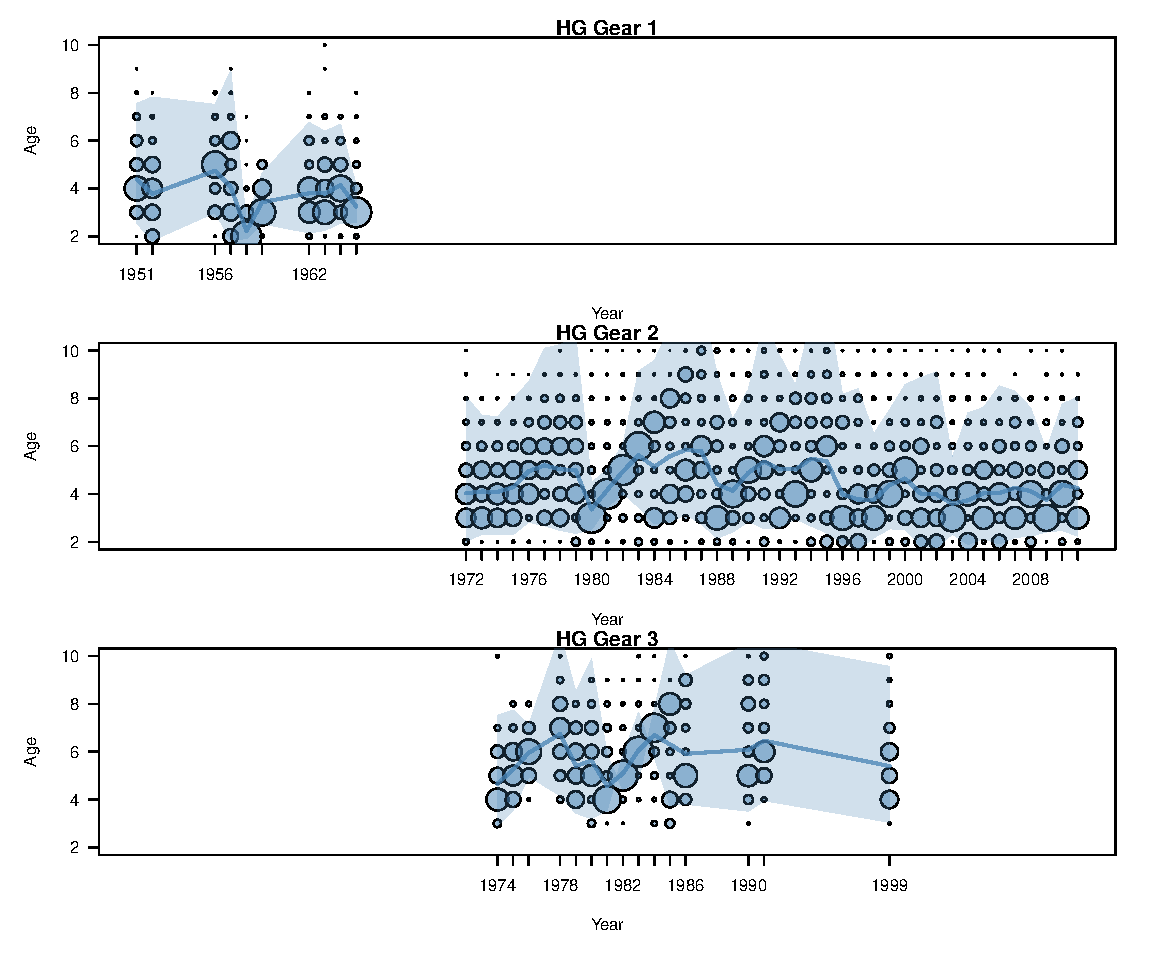
\includegraphics[width=0.85\textwidth]{../Figs/iscam_fig_AgeCompsHG.pdf}\\
	\caption{Bubble plots showing the proportions-at-age versus time for the winter purse seine fishery (top), seine roe fishery (middle) and the gillnet fishery (bottom) in Haida Gwaii.  The area of the circle is proportional to cohort abundance, each column sums to 1, zeros are not shown, and age 10 is a plus group. Also shown is the mean age of the catch (line) and the approximate 95\% distribution of ages (shaded polygon) for each year.}\label{FigAgeCompsHG}
\end{sidewaysfigure}

\begin{sidewaysfigure}[!tbp]
	% Requires \usepackage{graphicx}
	\centering
	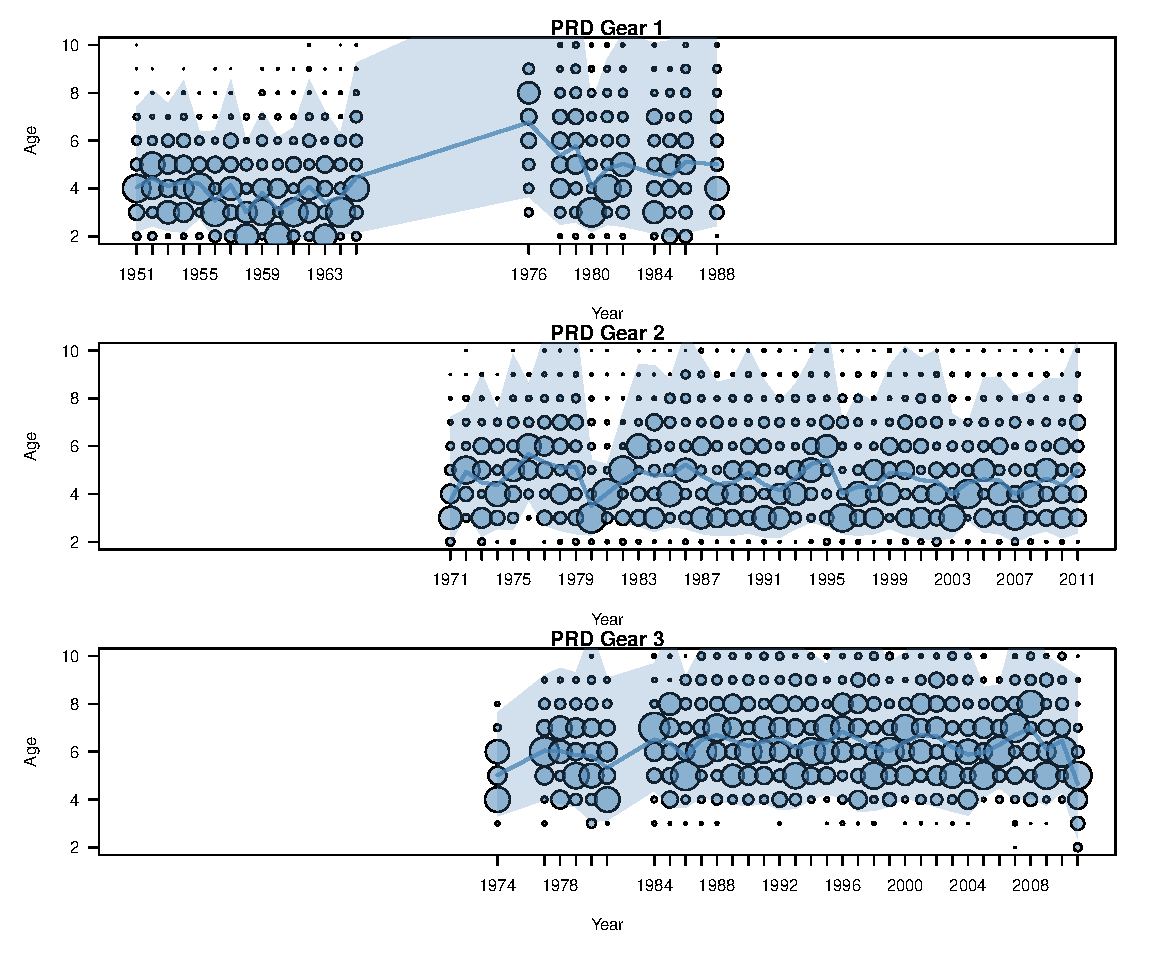
\includegraphics[width=0.85\textwidth]{../Figs/iscam_fig_AgeCompsPRD.pdf}\\
	\caption{Bubble plots showing the proportions-at-age versus time for the winter purse seine fishery (top), seine roe fishery (middle) and the gillnet fishery (bottom) in Prince Rupert District.  The area of the circle is proportional to cohort abundance, each column sums to 1, zeros are not shown, and age 10 is a plus group. Also shown is the mean age of the catch (line) and the approximate 95\% distribution of ages (shaded polygon) for each year.}\label{FigAgeCompsPRD}
\end{sidewaysfigure}

\begin{sidewaysfigure}[!tbp]
	% Requires \usepackage{graphicx}
	\centering
	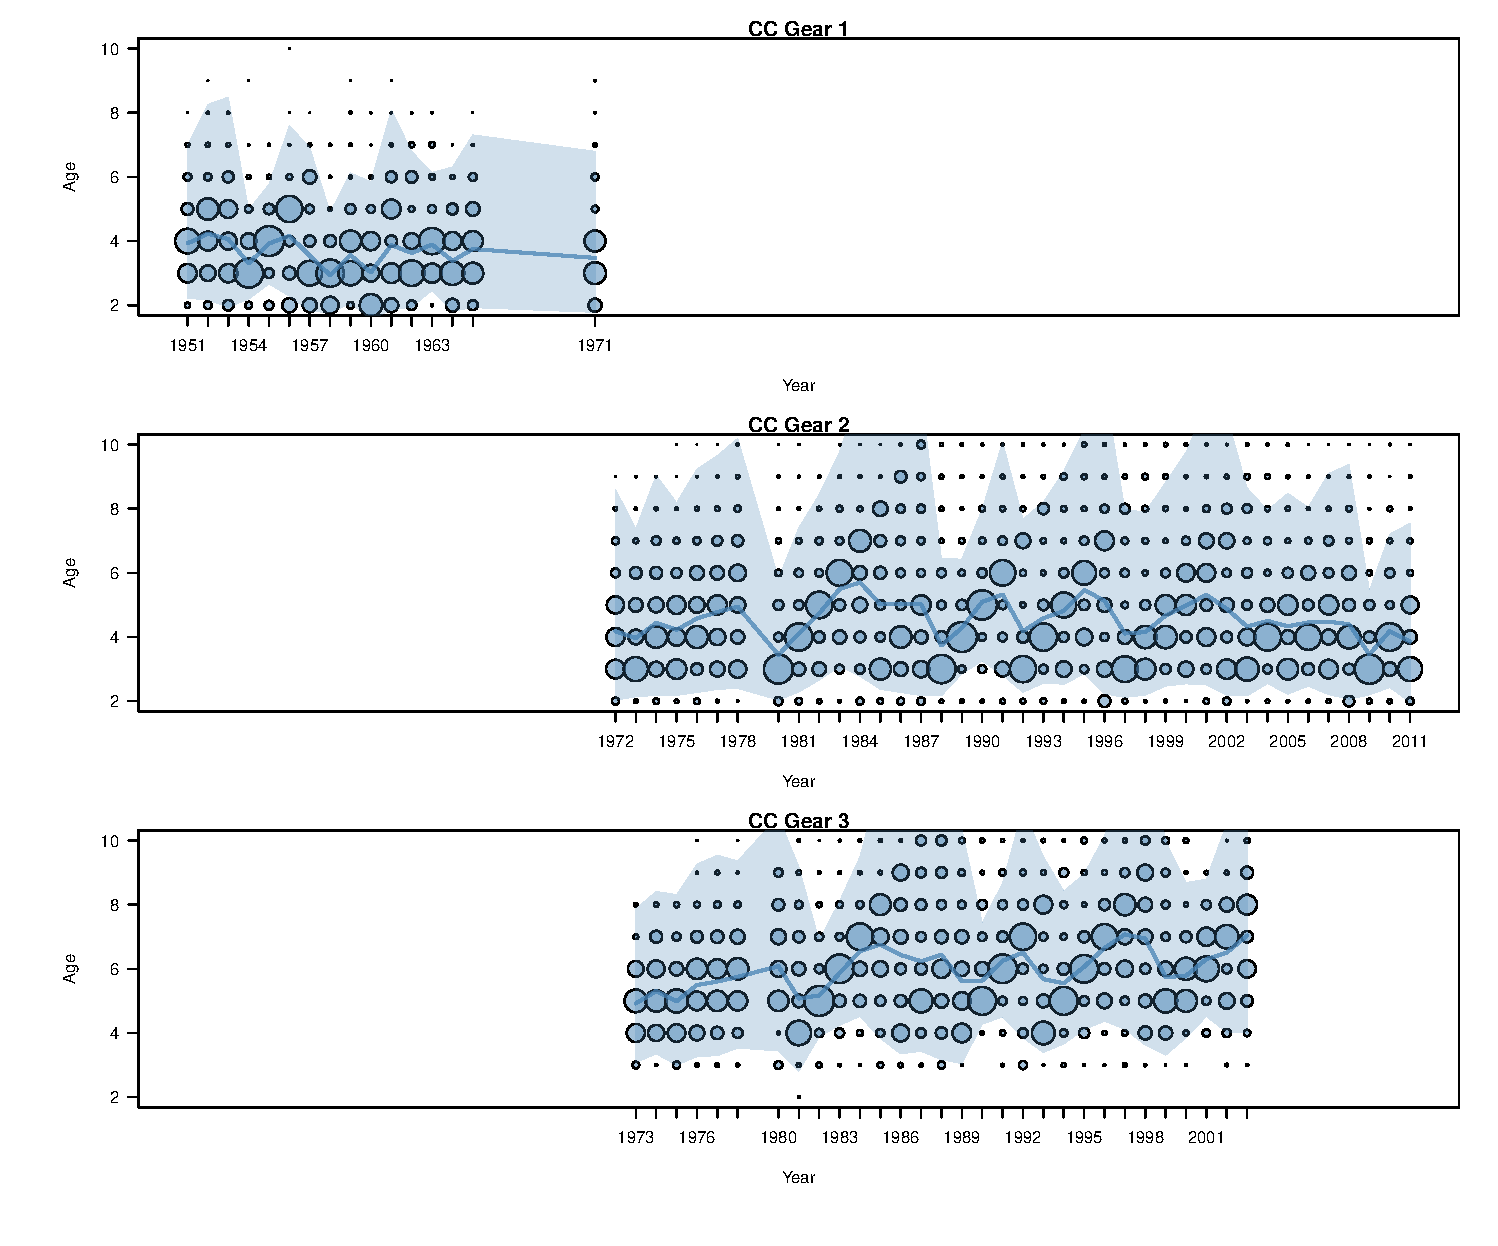
\includegraphics[width=0.85\textwidth]{../Figs/iscam_fig_AgeCompsCC.pdf}\\
	\caption{Bubble plots showing the proportions-at-age versus time for the winter purse seine fishery (top), seine roe fishery (middle) and the gillnet fishery (bottom) in the Central Coast region.  The area of the circle is proportional to cohort abundance, each column sums to 1, zeros are not shown, and age 10 is a plus group. Also shown is the mean age of the catch (line) and the approximate 95\% distribution of ages (shaded polygon) for each year.}\label{FigAgeCompsCC}
\end{sidewaysfigure}

\begin{sidewaysfigure}[!tbp]
	% Requires \usepackage{graphicx}
	\centering
	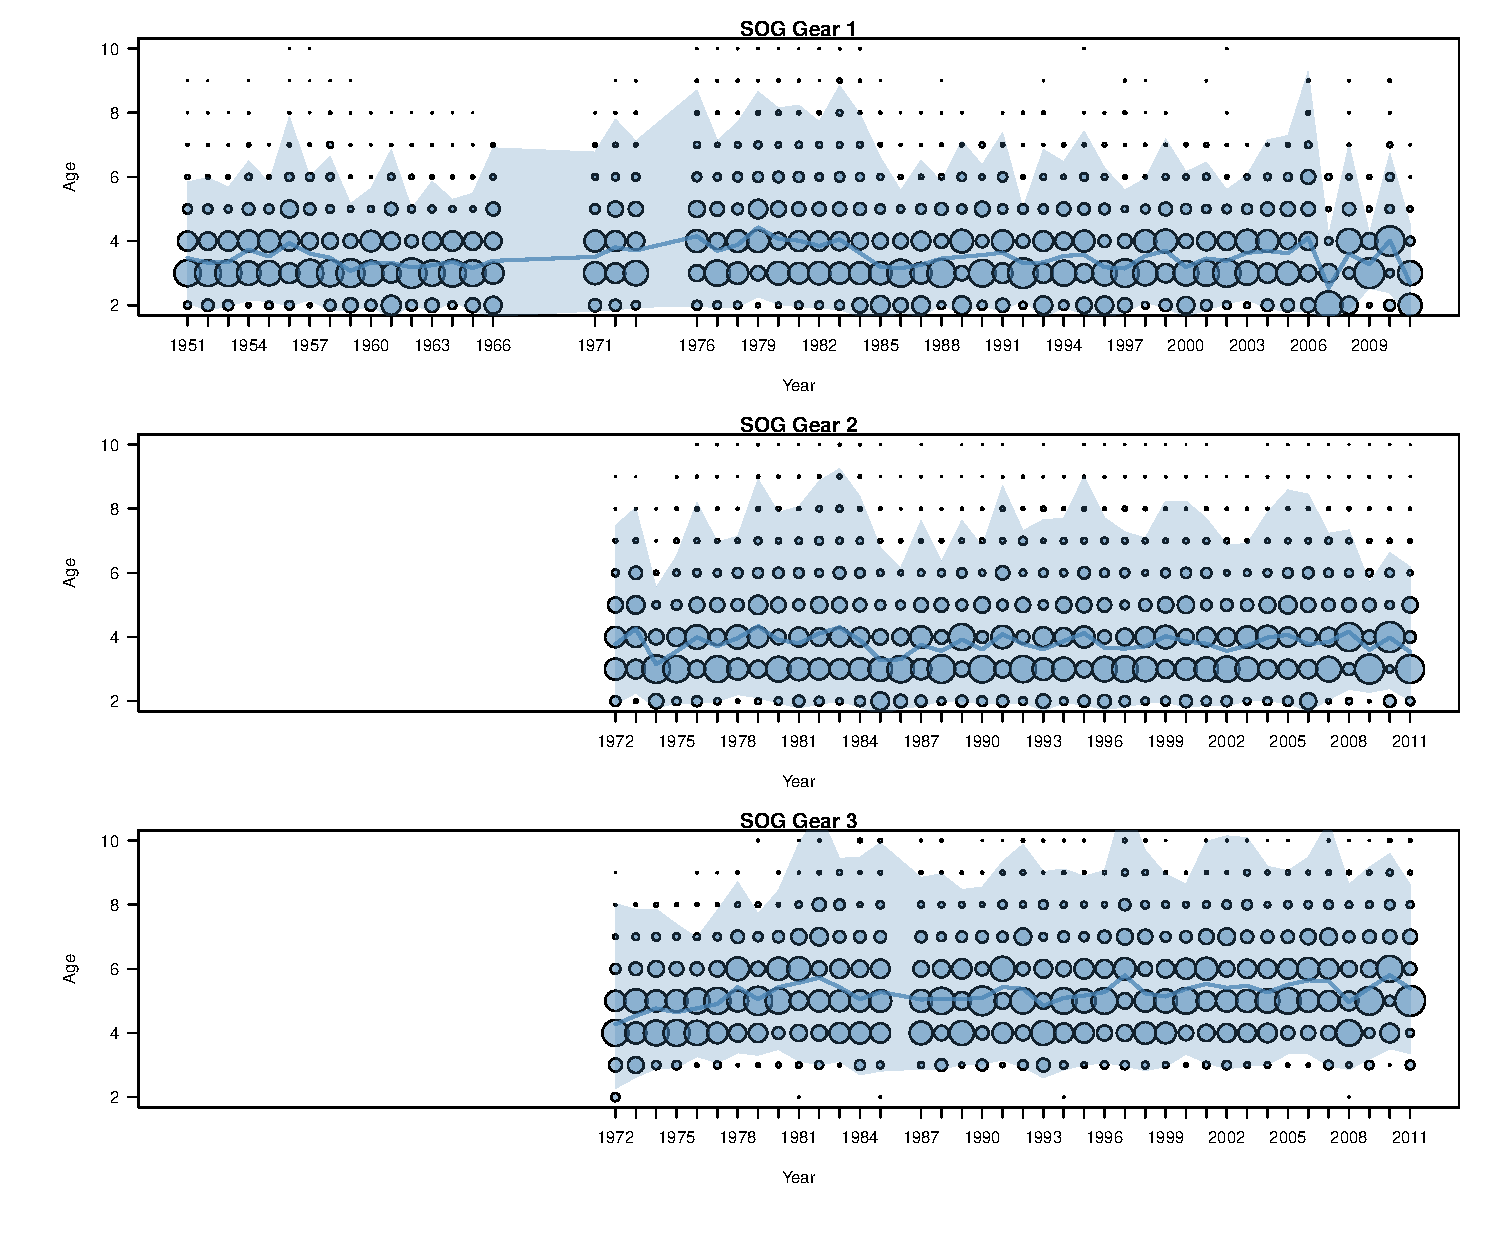
\includegraphics[width=0.85\textwidth]{../Figs/iscam_fig_AgeCompsSOG.pdf}\\
	\caption{Bubble plots showing the proportions-at-age versus time for the winter purse seine fishery (top), seine roe fishery (middle) and the gillnet fishery (bottom) in the Strait of Georgia.  The area of the circle is proportional to cohort abundance, each column sums to 1, zeros are not shown, and age 10 is a plus group. Also shown is the mean age of the catch (line) and the approximate 95\% distribution of ages (shaded polygon) for each year.}\label{FigAgeCompsSOG}
\end{sidewaysfigure}

\begin{sidewaysfigure}[!tbp]
	% Requires \usepackage{graphicx}
	\centering
	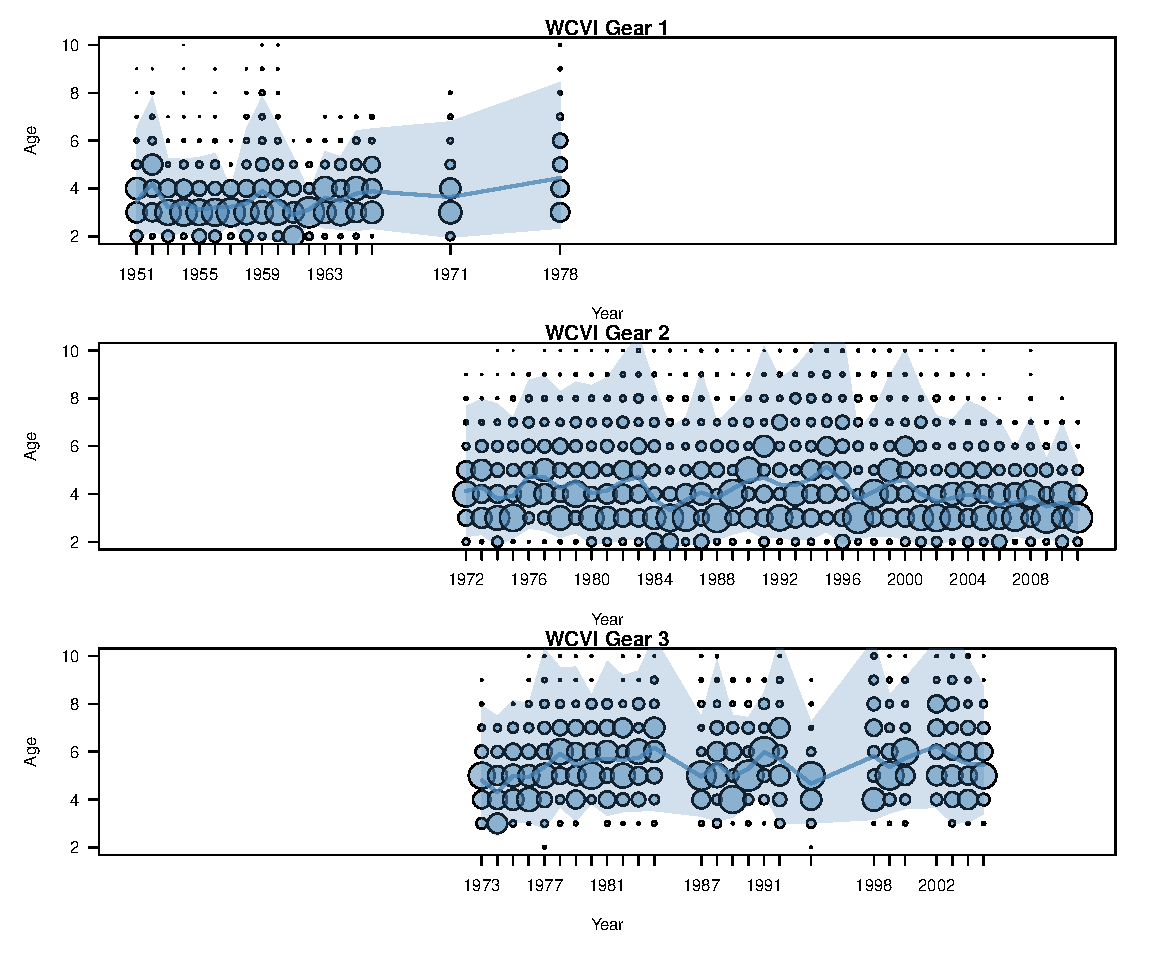
\includegraphics[width=0.85\textwidth]{../Figs/iscam_fig_AgeCompsWCVI.pdf}\\
	\caption{Bubble plots showing the proportions-at-age versus time for the winter purse seine fishery (top), seine roe fishery (middle) and the gillnet fishery (bottom) in the West Coast Vancouver Island region.  The area of the circle is proportional to cohort abundance, each column sums to 1, zeros are not shown, and age 10 is a plus group. Also shown is the mean age of the catch (line) and the approximate 95\% distribution of ages (shaded polygon) for each year.}\label{FigAgeCompsWCVI}
\end{sidewaysfigure}





	\subsubsection{Mean weight-at-age data}

	From the mid-1970s until the present, there has been a measurable decline in weight-at-age for all ages in all major stock areas (Figure \ref{FigMeanWt}). Samples collected during the 2009/10 fishing year indicate weights-at-age that are among the lowest on record. This declining weight-at-age may be attributed to any number of factors, including: fishing effects (i.e., gear selectivity), environmental effects (changes in ocean productivity), or it may even be attributed to changes in sampling protocols (shorter time frame over which samples are collected). Declining weight-at-age has been observed in all five of the major stocks, and despite area closures over the last 10-years, has continued to occur in the QCI and WCVI stocks. Although the direct cause of this decline is still to be investigated, this trend has been observed in B.C. and U.S. waters, from California to Alaska \citep{schweigert2002herring}, and merits further research.	The observed mean weight-at-age data appear to have a few  errors that need to be investigated as well; for example, see the apparently small age-10 fish in 2001 in Figure \ref{FigMeanWt}.

\begin{figure}[!tbp]
	% Requires \usepackage{graphicx}
	\centering
	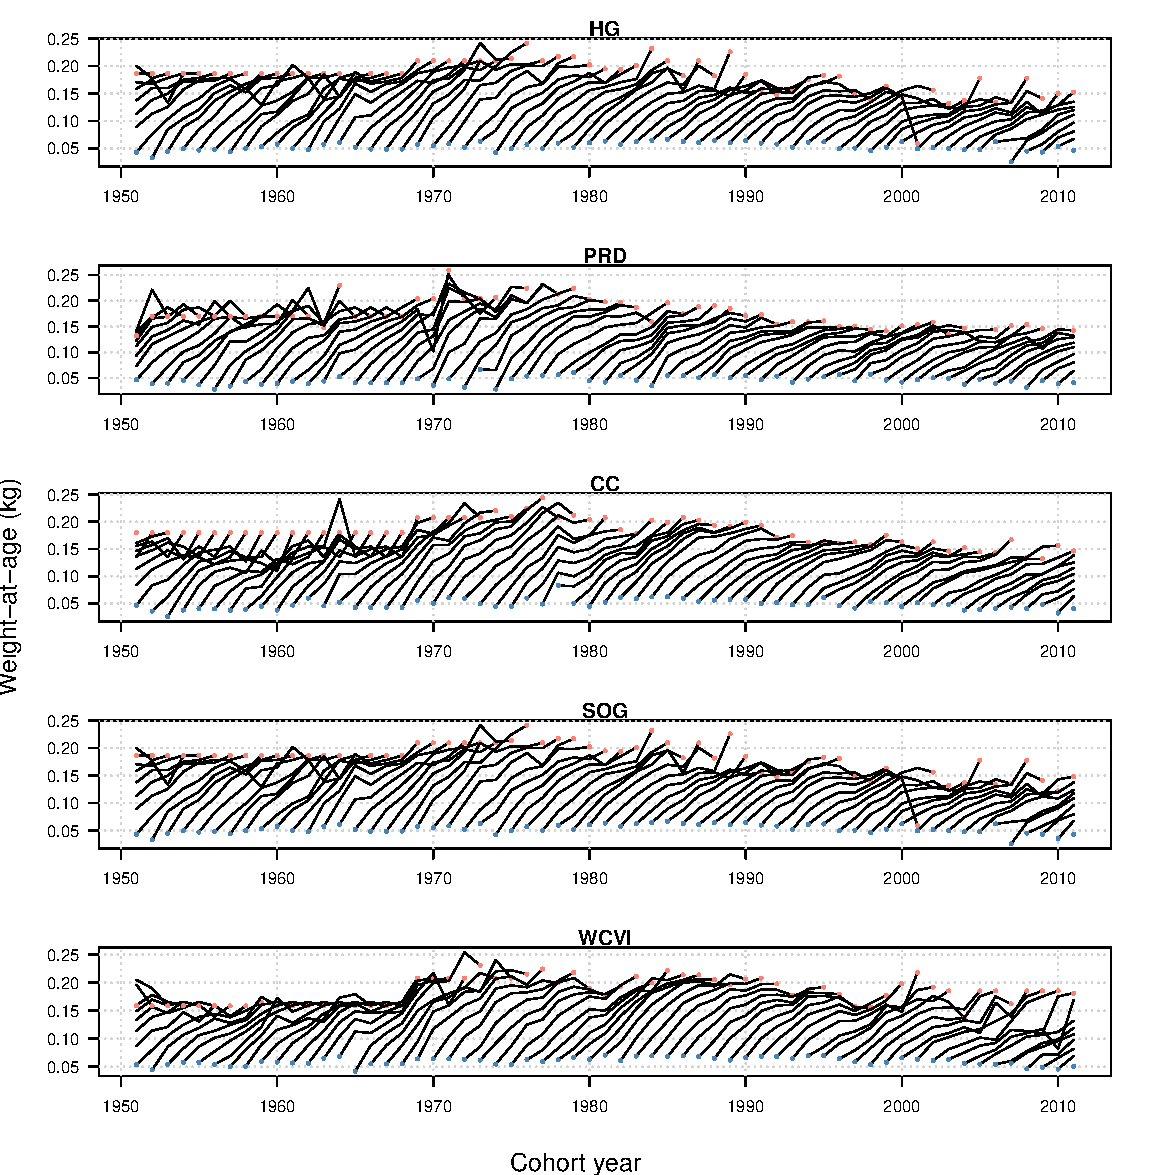
\includegraphics[width=\textwidth]{../Figs/iscam_fig_MeanWt.pdf}\\
	\caption{Empirical mean weight-at-age data by cohort from 1951 to 2011 for ages 2 to 10 in the five major Stock Assessment Regions.}\label{FigMeanWt}
\end{figure}
	

%%%%%%%%%%%%%%%%%%%%%%%%%%%%%%%%%%%%%%%%%%%%%%%%%%%%%%%%%%%%%%%%%%%%%
%%%%%%%%%%%%%%%%%%%%%%%%%%%%%%%%%%%%%%%%%%%%%%%%%%%%%%%%%%%%%%%%%%%%%
%%%%%%%%%%%%%%%%%%%%%%%%%%%%%%%%%%%%%%%%%%%%%%%%%%%%%%%%%%%%%%%%%%%%%	
	\subsection{Analytical methods}

	For the 2011 BC herring assessment, \iscam was used to conduct the stock assessment for each of the five major Stock Assessment Regions (SAR) and two minor assessment areas (Area 2W and Area 27).  The technical details of this model can be found in Appendix \ref{appiSCAM}.
		
	\subsection{Retrospective analysis}
	A retrospective analysis was conducted for each of the major and minor SARs.  The retrospective analysis successively removes the last 10-years of data and examines changes in estimates of terminal spawning biomass.  The results are then plotted on a single panel to compare how estimates of spawning biomass change as successive years of data are omitted from the analysis.
	
	\subsection{Abundance and recruitment forecasts}
	The abundance forecast for the upcoming fishing season, also referred to as pre-fishery biomass, is defined as the predicted biomass of age-4 fish and older plus the number of age-3 fish recruiting in year $T+1$.  The abundance estimates are based on the median values from the sampled posterior distribution.  Age-3 recruits are based on poor, average, and good recruitment scenarios; see next paragraph for definitions of poor, average and good.
	
	The recruitment forecasts are based on the surviving number of age-3 fish at the start of the fishing season times the average weight-at-age 3 in the last 5 years. The definitions of poor, average, and good recruitment are as follows: \textbf{Poor} is the average recruitment from the 0-33 percentile, \textbf{Average} is the average recruitment from the 33-66 percentile, and \textbf{Good} is the average recruitment from the 66-100 percentile.  Note that all cohorts from 1951 to 2011  were included in the calculation of recruitment quantiles.
	
	\subsection{Catch advice}
Catch advice is based on the application of the harvest control rule (HCR). The herring HCR has three components:
\begin{enumerate}
\item Reference points (LRP, USR, and cuttoffs)
\item Harvest rate
\item Decision rules
\end{enumerate}

For each of the five major stocks, the limit reference point (LRP) is the cuttoff value, which is defined here as 0.25\bo\, and the	Upper Stock Reference (USR) is defined as the 1.05*LRP (0.25\bo\ + 0.2*0.25\bo = LRP + 0.05LRP). \textbf{For clarification, references to \bo\ throughout this document refer to the mature spawning stock biomass.} The default harvest rate if the stock is at or above USR is 0.2, and declines linearly to 0 when the stock is at or below the LRP (a default harvest rate of 0.1 is used for the minor stock areas).  The decision rule for the major stock areas operates as follows:

\begin{itemize}
	\item If the forecast run is less than the LRP (cuttoff) then the area is closed to all commercial harvest  (i.e., stock is deemed to be in the critical zone).
	
	\item If the forecast run is greater than the LRP and less than the USR (i.e., cautious zone), then total allowable catch is based on a reduced harvest rate that would deplete the stock to the LRP level.
	
	\item If the forecast run is greater than USR, then the total allowable catch is set at 20\% of the forecast run.
\end{itemize}



	






%% -End of main body of the document------------------------------------

  %% -References
\clearpage
%input "Refs.bib"
%\bibliographystyle{plainnat}
\addcontentsline{toc}{section}{References}
\bibliographystyle{apalike}
\bibliography{$HOME/Documents/ARTICLES/Articles-1}


%% Appendices
\part{Appendices}
%\setcounter{chapter}{1}
\appendix

\addtocounter{section}{0}
\renewcommand{\thetable}{A-\arabic{table}}
\setcounter{table}{0}
\setcounter{chapter}{1}
%!TEX root = /Users/stevenmartell/Documents/iSCAM-project/fba/Halibut/WRITEUP/Halibut.tex


\section{Input files for the Simulation Model} \label{appen:dataFiles}

In this appendix, the input data, parameter controls and initial parameter values for the Halibut simulation model are given.  Electronic copies of these files are available from a code repository hosted at: \url{http://code.google.com/p/iscam-project/source/browse/}.  The source code is also available from the same repository under the Halibut branch.  A history of the code development can be viewed here: \url{http://code.google.com/p/iscam-project/source/list?name=halibut}.


The following is the data file where, the \# symbol to the left of any number denotes comment lines to document the data file.


\tiny
\begin{alltt}
\input{../DATA/Halibut_2sex_develop.dat}
\end{alltt}
\normalsize


The following text is the control file for the halibut simulation model
\tiny
\begin{alltt}
\input{../DATA/Halibut_2sex_develop.ctl}
\end{alltt}
\normalsize


\tiny
\begin{alltt}
\input{../DATA/Halibut_2sex_develop.pin}
\end{alltt}
\normalsize

\setcounter{chapter}{2}
%!TEX root = /Users/stevenmartell/Documents/iSCAM-project/fba/Halibut/WRITEUP/Halibut.tex

\section{Model Description} % (fold)
\label{sec:model_description}

The following detailed documentation is a description of the simulation model used to generate model output in this report.  The description is broken down into three subsections: 1) simulation model input, 2) state dynamics, and 3) model outputs.  A series of tables along with a detailed written description is used to document the model.  The tables of equations are meant to represent the logical progression of using input data to initialize the population model, simulating dynamical responses to alternative policies and deriving model outputs.

To summarize the following subsections that describe the model in detail, the following pseudocode represents the general order of operations (implemented as specific functions within the computer code).

\noindent\underline{Pseudocode:}
\begin{enumerate}
	\item Read simulation model inputs, (biological data, fishery data and model parameters).
	\item Initialize model parameters (initial age-structure, annual recruitment, etc).
	\item Calculate length-based selectivities for each gear type for each sex.
	\item Partition fishing mortality to each fishing sector.
	\item Calculate age-specific total mortality rate for each year where the probability of capture and discard is a function of selectivity and size limits.
	\item Calculate numbers-at-age each year based on annual values of $Z$.
	\item Compute model outputs and performance measures.
\end{enumerate}

% -----------------------------------------------------------------------------
\subsection{Simulation model input} % (fold)
\label{sub:simulation_model_input}

List of model input:
\begin{enumerate}
	\item Historical catch data, or fishing mortality rates.
	\item Annual recruitment from 1996 to present.
	\item Initial numbers-at-age by sex.
	\item Stock parameters ($B_0$,$h$,$M$)
	\item Selectivity parameters (length-based selectivity)
	\item Size limit, target harvest rate, \& other policy related parameters (e.g., SUFD).
\end{enumerate}

\begin{table}[ht]
	\caption{List of symbols, units and description of variables for the simulation model.}
	\label{tab:ListOfSymbols}
	\begin{center}
	\begin{tabular}{ccl}
		\hline
		Symbol & Units & Description \\
		\hline
		$h$	& - & index for sex\\
		$i$	& - & index for year\\
		$j$	& - & index for age\\
		$k$	& - & index for gear\\
		\multicolumn{3}{l}{\underline{Input Parameters}}\\
		$R_0$	& millions	& unfished recruitment\\
		$h$		& -			& steepness of the stock-recruitment relationship\\
		$M_h$	& yr$^{-1}$	& instantaneous natural mortality rate by sex \\
		$\bar{R}$ & millions & average recruitment\\
		$\ddot{R}$ & millions & initial recruitment\\
		$\omega_i$ & - & annual recruitment deviation in year i\\
		$\ddot{\omega_j}$ & - & initial recruitment deviation for age j\\
		\hline
	\end{tabular}
	\end{center}
\end{table}

% subsection simulation_model_input (end)
% -----------------------------------------------------------------------------
\subsection{Analytical description} % (fold)
\label{sub:analytical_description}

% 1) Initial states
% 2) Selectivities and joint probablity for fishing mortality & discard mortality.
% 3) Calculating fishing mortality rates from 1994-present conditioned on catch.
In the more recent stock assessment models, the age/sex/size composition of the commercial landings are estimated externally to the model.  These data are not readily available to be used in this analysis.  The sex composition of the commercial catch was approximated by applying the same fishing mortality rate to each of the sexes, where the fishing mortality rate was approximated by the historical total landings divided by the simulated exploitable biomass (both sexes combined).  This differs substantially from the methods used to apportion commercial catch to each sex \cite[see][for details]{clark2004method}.


% 4) Calculate sex- age-specifc total mortality rates

% subsection analytical_description (end)
% -----------------------------------------------------------------------------
\subsection{Model outputs} % (fold)
\label{sub:model_outputs}

% subsection model_outputs (end)


% section model_description (end)


\end{document}
